\documentclass[sigconf,nonacm]{acmart}
\usepackage{pvldb}
\usepackage{algorithm}
\usepackage{algpseudocode}
\usepackage{multirow}
\usepackage{makecell}
\usepackage{tikz}
\usetikzlibrary{arrows.meta,positioning,fit,calc}
% generated by paper/pvldb/make_numbers.py -- do not edit
\newcommand{\Nbirddebhit}{99.5}
\newcommand{\Nbirddebn}{64}
\newcommand{\Nbirddebref}{41.5}
\newcommand{\Nbirddebsame}{yes}
\newcommand{\Nbirddebstat}{41.5}
\newcommand{\Nbirddebstrict}{41.5}
\newcommand{\Nbirdfinhit}{88.5}
\newcommand{\Nbirdfinn}{106}
\newcommand{\Nbirdfinref}{19.6}
\newcommand{\Nbirdfinsame}{yes}
\newcommand{\Nbirdfinstat}{19.6}
\newcommand{\Nbirdfinstrict}{21.8}
\newcommand{\Nconcms}{4.6}
\newcommand{\Nconcq}{50}
\newcommand{\Nconcsess}{8}
\newcommand{\Ndpauditatt}{11.5}
\newcommand{\Ndpauditn}{200}
\newcommand{\Ndpauditnarrow}{0}
\newcommand{\Ndpauditprior}{11.5}
\newcommand{\Ndpauditwidth}{11000}
\newcommand{\Ndphundredatt}{11.2}
\newcommand{\Ndphundrederr}{1.8}
\newcommand{\Ndphundrederrpct}{1.8}
\newcommand{\Ndphundredfive}{77.4}
\newcommand{\Ndphundredsup}{0.0}
\newcommand{\Ndphundredsupn}{29}
\newcommand{\Ndponeatt}{0.1}
\newcommand{\Ndponeerr}{148.0}
\newcommand{\Ndponeerrpct}{148.0}
\newcommand{\Ndponefive}{5.6}
\newcommand{\Ndponesup}{25.2}
\newcommand{\Ndponesupn}{21145}
\newcommand{\Ndptenatt}{1.1}
\newcommand{\Ndptenerr}{17.3}
\newcommand{\Ndptenerrpct}{17.3}
\newcommand{\Ndptenfive}{25.1}
\newcommand{\Ndptensup}{2.0}
\newcommand{\Ndptensupn}{1696}
\newcommand{\Neechk}{1.4}
\newcommand{\Neechkproxy}{1.8}
\newcommand{\Neeexe}{11.5}
\newcommand{\Neeexecn}{2616}
\newcommand{\Neemax}{4.44}
\newcommand{\Neen}{2942}
\newcommand{\Neeover}{112}
\newcommand{\Neertexec}{53.7}
\newcommand{\Neesummed}{14.0}
\newcommand{\Nexfouradm}{56.3}
\newcommand{\Nexfouradmn}{197}
\newcommand{\Nexfourall}{50.5}
\newcommand{\Nexfourn}{220}
\newcommand{\Nexminiadm}{57.8}
\newcommand{\Nexminiadmn}{154}
\newcommand{\Nexminiall}{40.5}
\newcommand{\Nexminin}{220}
\newcommand{\Nexqwenadm}{42.2}
\newcommand{\Nexqwenadmn}{45}
\newcommand{\Nexqwenall}{34.5}
\newcommand{\Nexqwenn}{55}
\newcommand{\Nexsonnetadm}{69.8}
\newcommand{\Nexsonnetadmn}{202}
\newcommand{\Nexsonnetall}{64.1}
\newcommand{\Nexsonnetn}{220}
\newcommand{\Nfloatdisagree}{0}
\newcommand{\Nfloatsearchdisagree}{0}
\newcommand{\Nfloattoler}{1e-9}
\newcommand{\Nfloattrials}{400}
\newcommand{\Nhistcust}{1,000,000}
\newcommand{\Nhistmax}{3.71}
\newcommand{\Nhistmed}{1.02}
\newcommand{\Nhistn}{1000}
\newcommand{\Nhistover}{0}
\newcommand{\Nhistrank}{1000}
\newcommand{\Nktenlinearq}{20.1}
\newcommand{\Nktenlinears}{89.5}
\newcommand{\Nktenlinearsmall}{100.0}
\newcommand{\Nktenlinearthree}{100.0}
\newcommand{\Nktenlineartwo}{100.0}
\newcommand{\Nktenpairwiseq}{20.1}
\newcommand{\Nktenpairwises}{89.5}
\newcommand{\Nktenpairwisesmall}{100.0}
\newcommand{\Nktenpairwisethree}{83.0}
\newcommand{\Nktenpairwisetwo}{100.0}
\newcommand{\Nktenstatelessq}{20.1}
\newcommand{\Nktenstatelesss}{89.5}
\newcommand{\Nktenstatelesssmall}{100.0}
\newcommand{\Nktenstatelessthree}{82.0}
\newcommand{\Nktenstatelesstwo}{76.0}
\newcommand{\Nktenstrictq}{37.3}
\newcommand{\Nktenstricts}{97.8}
\newcommand{\Nktenstrictsmall}{100.0}
\newcommand{\Nktenstrictthree}{100.0}
\newcommand{\Nktenstricttwo}{100.0}
\newcommand{\Nkthreelinearq}{3.3}
\newcommand{\Nkthreelinears}{26.8}
\newcommand{\Nkthreelinearsmall}{100.0}
\newcommand{\Nkthreelinearthree}{100.0}
\newcommand{\Nkthreelineartwo}{100.0}
\newcommand{\Nkthreenq}{4366}
\newcommand{\Nkthreens}{400}
\newcommand{\Nkthreepairwiseq}{3.3}
\newcommand{\Nkthreepairwises}{26.8}
\newcommand{\Nkthreepairwisesmall}{100.0}
\newcommand{\Nkthreepairwisethree}{12.0}
\newcommand{\Nkthreepairwisetwo}{100.0}
\newcommand{\Nkthreestatelessq}{0.6}
\newcommand{\Nkthreestatelesss}{7.0}
\newcommand{\Nkthreestatelesssmall}{100.0}
\newcommand{\Nkthreestatelessthree}{3.0}
\newcommand{\Nkthreestatelesstwo}{1.0}
\newcommand{\Nkthreestrictq}{25.6}
\newcommand{\Nkthreestricts}{94.0}
\newcommand{\Nkthreestrictsmall}{100.0}
\newcommand{\Nkthreestrictthree}{100.0}
\newcommand{\Nkthreestricttwo}{100.0}
\newcommand{\Nnaivehundredatt}{18.7}
\newcommand{\Nnaivehundrederr}{0.9}
\newcommand{\Nnaiveoneatt}{0.1}
\newcommand{\Nnaiveoneerr}{87.7}
\newcommand{\Nnaivetenatt}{2.2}
\newcommand{\Nnaivetenerr}{8.8}
\newcommand{\Npairkthreeadm}{0}
\newcommand{\Npairn}{100}
\newcommand{\Npairnoneadm}{100}
\newcommand{\Npairnoneexact}{0}
\newcommand{\Npairnonesum}{100}
\newcommand{\Nscalecell}{3.0}
\newcommand{\Nscalejoin}{14.2}
\newcommand{\Nscalenation}{40,000}
\newcommand{\Nscaleship}{6.0}
\newcommand{\Nscaleweights}{9.4}
\newcommand{\Nsearchbudget}{100}
\newcommand{\Nsearchexactkthree}{0}
\newcommand{\Nsearchexactkthreebis}{0}
\newcommand{\Nsearchlinearkfive}{0}
\newcommand{\Nsearchlinearkfivebis}{0}
\newcommand{\Nsearchlinearkten}{0}
\newcommand{\Nsearchlinearktenbis}{0}
\newcommand{\Nsearchlinearkthree}{0}
\newcommand{\Nsearchlinearkthreebis}{0}
\newcommand{\Nsearchn}{100}
\newcommand{\Nsearchnone}{100}
\newcommand{\Nsearchnonebis}{100}
\newcommand{\Nsearchpairwisekthree}{100}
\newcommand{\Nsearchpairwisekthreebis}{0}
\newcommand{\Nsearchstatelesskfive}{100}
\newcommand{\Nsearchstatelesskfivebis}{100}
\newcommand{\Nsearchstatelesskten}{100}
\newcommand{\Nsearchstatelessktenbis}{100}
\newcommand{\Nsearchstatelesskthree}{100}
\newcommand{\Nsearchstatelesskthreebis}{100}
\newcommand{\Nsearchstrictkthree}{0}
\newcommand{\Nsearchstrictkthreebis}{0}
\newcommand{\Nsearchwilson}{3.7}

\newcommand{\Nfinrefsplit}{16.6}
\newcommand{\Nfinsinglesplit}{16}
\newcommand{\Nfinhitsplit}{82.0}
\newcommand{\Ndebitrefsplit}{37.3}
\newcommand{\Ndebitsinglesplit}{24}
\newcommand{\Ndebithitsplit}{99.5}

\newcommand{\Nprogn}{200}
\newcommand{\Nprognthresh}{50}
\newcommand{\Nprogthreshq}{132}
\newcommand{\Npairbenign}{3.3}
\newcommand{\Nlinbenign}{3.3}
\newcommand{\Npairmed}{2.2}
\newcommand{\Nlinmed}{1.9}
\newcommand{\Nrankmed}{126}
\newcommand{\Nrankmax}{135}
\newcommand{\Nbirdrefn}{40}
\newcommand{\Nbirddesign}{30}
\newcommand{\Nbirdfp}{7}
\newcommand{\Nbirdborder}{3}
\newcommand{\Nbirdfpfan}{5}
\newcommand{\Nfinrefpair}{16.6}
\newcommand{\Ndebitrefpair}{37.3}
\newcommand{\Nfisherm}{0.11}
\newcommand{\Npairrefm}{3.9}
\newcommand{\Nfishero}{0.46}
\newcommand{\Npairrefo}{2.3}
\newcommand{\Nfinmlpn}{50}
\newcommand{\Nfinmlpdisc}{0}
\newcommand{\Nfinmlppair}{0}
\newcommand{\Nfinmlphi}{7.1}
\newcommand{\Nfinmlpref}{6.5}
\newcommand{\Nfinmlpq}{14.9}
\newcommand{\Nfinmlpdecl}{0}
\newcommand{\Nfinmspn}{50}
\newcommand{\Nfinmspdisc}{0}
\newcommand{\Nfinmsppair}{0}
\newcommand{\Nfinmsphi}{7.1}
\newcommand{\Nfinmspref}{6.7}
\newcommand{\Nfinmspq}{14.9}
\newcommand{\Nfinmspdecl}{0}
\newcommand{\Nfinolpn}{25}
\newcommand{\Nfinolpdisc}{0}
\newcommand{\Nfinolppair}{0}
\newcommand{\Nfinolphi}{13.3}
\newcommand{\Nfinolpref}{3.8}
\newcommand{\Nfinolpq}{9.8}
\newcommand{\Nfinolpdecl}{0}
\newcommand{\Nfinospn}{25}
\newcommand{\Nfinospdisc}{0}
\newcommand{\Nfinosppair}{0}
\newcommand{\Nfinosphi}{13.3}
\newcommand{\Nfinospref}{3.9}
\newcommand{\Nfinospq}{9.8}
\newcommand{\Nfinospdecl}{0}

\newcommand{\Nsupthreelinref}{3.3}
\newcommand{\Nsupthreelinmed}{1.9}
\newcommand{\Nsupthreelinp}{18}
\newcommand{\Nsupthreepairref}{3.3}
\newcommand{\Nsupthreepairmed}{2.1}
\newcommand{\Nsupthreepairp}{24}
\newcommand{\Nsupthreecombref}{3.3}
\newcommand{\Nsupthreecombmed}{2.4}
\newcommand{\Nsupthreecombp}{25}
\newcommand{\Nsupfourlinref}{4.8}
\newcommand{\Nsupfourlinmed}{2.0}
\newcommand{\Nsupfourlinp}{18}
\newcommand{\Nsupfourpairref}{4.8}
\newcommand{\Nsupfourpairmed}{2.2}
\newcommand{\Nsupfourpairp}{24}
\newcommand{\Nsupfourcombref}{4.8}
\newcommand{\Nsupfourcombmed}{2.2}
\newcommand{\Nsupfourcombp}{24}
\newcommand{\Nsupfivelinref}{13.9}
\newcommand{\Nsupfivelinmed}{1.7}
\newcommand{\Nsupfivelinp}{5}
\newcommand{\Nsupfivepairref}{13.9}
\newcommand{\Nsupfivepairmed}{1.9}
\newcommand{\Nsupfivepairp}{6}
\newcommand{\Nsupfivecombref}{13.9}
\newcommand{\Nsupfivecombmed}{1.9}
\newcommand{\Nsupfivecombp}{6}
\newcommand{\Nsupn}{200}

\newcommand{\Nagpromptadmlost}{16}
\newcommand{\Nagpromptadmwon}{5}
\newcommand{\Nagpromptadmp}{0.03}
\newcommand{\Nagpromptadmfrom}{53}
\newcommand{\Nagpromptadmto}{45}
\newcommand{\Nagadmn}{134}
\newcommand{\Nagpromptonelost}{3}
\newcommand{\Nagpromptonewon}{3}
\newcommand{\Nagpromptonep}{1.00}
\newcommand{\Nagpromptonefrom}{44}
\newcommand{\Nagpromptoneto}{44}
\newcommand{\Nagonen}{27}
\newcommand{\Naggateadmlost}{4}
\newcommand{\Naggateadmwon}{1}
\newcommand{\Naggateadmp}{0.38}
\newcommand{\Naggateadmfrom}{45}
\newcommand{\Naggateadmto}{43}
\newcommand{\Naggateonelost}{11}
\newcommand{\Naggateonewon}{0}
\newcommand{\Naggateonep}{$<$0.01}
\newcommand{\Naggateonefrom}{44}
\newcommand{\Naggateoneto}{4}
\newcommand{\Naggatenradmlost}{5}
\newcommand{\Naggatenradmwon}{2}
\newcommand{\Naggatenradmp}{0.45}
\newcommand{\Naggatenradmfrom}{53}
\newcommand{\Naggatenradmto}{51}
\newcommand{\Naggatenronelost}{12}
\newcommand{\Naggatenronewon}{0}
\newcommand{\Naggatenronep}{$<$0.01}
\newcommand{\Naggatenronefrom}{44}
\newcommand{\Naggatenroneto}{0}
\newcommand{\Nsppromptothlost}{2}
\newcommand{\Nsppromptothwon}{2}
\newcommand{\Nsppromptothp}{1.00}
\newcommand{\Nsppromptothfrom}{12}
\newcommand{\Nsppromptothto}{12}
\newcommand{\Nspothn}{48}
\newcommand{\Nsppromptentlost}{0}
\newcommand{\Nsppromptentwon}{0}
\newcommand{\Nsppromptentp}{1.00}
\newcommand{\Nsppromptentfrom}{0}
\newcommand{\Nsppromptentto}{0}
\newcommand{\Nspentn}{12}
\newcommand{\Nspgatenrothlost}{3}
\newcommand{\Nspgatenrothwon}{1}
\newcommand{\Nspgatenrothp}{0.62}
\newcommand{\Nspgatenrothfrom}{12}
\newcommand{\Nspgatenrothto}{8}
\newcommand{\Nspgatenrentlost}{0}
\newcommand{\Nspgatenrentwon}{0}
\newcommand{\Nspgatenrentp}{1.00}
\newcommand{\Nspgatenrentfrom}{0}
\newcommand{\Nspgatenrentto}{0}
\newcommand{\Nspothref}{2.5}
\newcommand{\Nspothopenc}{6}
\newcommand{\Nspothgatec}{4}
\newcommand{\Nspentref}{6.8}
\newcommand{\Nspentopenc}{0}
\newcommand{\Nspentgatec}{0}
\newcommand{\Nspn}{60}
\newcommand{\Nspdbs}{13}
\newcommand{\Nspcatpolicy}{31}
\newcommand{\Nspcatshape}{35}
\newcommand{\Nspcataudit}{34}
\newcommand{\Nspnref}{203}
\newcommand{\Nsplost}{3}
\newcommand{\Nsplostshape}{3}
\newcommand{\Nsspromptothlost}{4}
\newcommand{\Nsspromptothwon}{4}
\newcommand{\Nsspromptothp}{1.00}
\newcommand{\Nsspromptothfrom}{56}
\newcommand{\Nsspromptothto}{56}
\newcommand{\Nssothn}{48}
\newcommand{\Nsspromptentlost}{0}
\newcommand{\Nsspromptentwon}{2}
\newcommand{\Nsspromptentp}{0.50}
\newcommand{\Nsspromptentfrom}{67}
\newcommand{\Nsspromptentto}{83}
\newcommand{\Nssentn}{12}
\newcommand{\Nssgatenrothlost}{10}
\newcommand{\Nssgatenrothwon}{1}
\newcommand{\Nssgatenrothp}{0.01}
\newcommand{\Nssgatenrothfrom}{56}
\newcommand{\Nssgatenrothto}{38}
\newcommand{\Nssgatenrentlost}{6}
\newcommand{\Nssgatenrentwon}{0}
\newcommand{\Nssgatenrentp}{0.03}
\newcommand{\Nssgatenrentfrom}{67}
\newcommand{\Nssgatenrentto}{17}
\newcommand{\Nssothref}{0.8}
\newcommand{\Nssothopenc}{27}
\newcommand{\Nssothgatec}{18}
\newcommand{\Nssentref}{2.1}
\newcommand{\Nssentopenc}{8}
\newcommand{\Nssentgatec}{2}
\newcommand{\Nssn}{60}
\newcommand{\Nssdbs}{13}
\newcommand{\Nsscatpolicy}{29}
\newcommand{\Nsscatshape}{45}
\newcommand{\Nsscataudit}{26}
\newcommand{\Nssnref}{62}
\newcommand{\Nsslost}{10}
\newcommand{\Nsslostshape}{8}
\newcommand{\Nsnpromptothlost}{4}
\newcommand{\Nsnpromptothwon}{4}
\newcommand{\Nsnpromptothp}{1.00}
\newcommand{\Nsnpromptothfrom}{56}
\newcommand{\Nsnpromptothto}{56}
\newcommand{\Nsnothn}{48}
\newcommand{\Nsnpromptentlost}{0}
\newcommand{\Nsnpromptentwon}{2}
\newcommand{\Nsnpromptentp}{0.50}
\newcommand{\Nsnpromptentfrom}{67}
\newcommand{\Nsnpromptentto}{83}
\newcommand{\Nsnentn}{12}
\newcommand{\Nsngatenrothlost}{8}
\newcommand{\Nsngatenrothwon}{1}
\newcommand{\Nsngatenrothp}{0.04}
\newcommand{\Nsngatenrothfrom}{56}
\newcommand{\Nsngatenrothto}{42}
\newcommand{\Nsngatenrentlost}{6}
\newcommand{\Nsngatenrentwon}{0}
\newcommand{\Nsngatenrentp}{0.03}
\newcommand{\Nsngatenrentfrom}{67}
\newcommand{\Nsngatenrentto}{17}
\newcommand{\Nsnothref}{0.5}
\newcommand{\Nsnothopenc}{27}
\newcommand{\Nsnothgatec}{20}
\newcommand{\Nsnentref}{1.2}
\newcommand{\Nsnentopenc}{8}
\newcommand{\Nsnentgatec}{2}
\newcommand{\Nsnn}{60}
\newcommand{\Nsndbs}{13}
\newcommand{\Nsncatpolicy}{46}
\newcommand{\Nsncatshape}{5}
\newcommand{\Nsncataudit}{49}
\newcommand{\Nsnnref}{39}
\newcommand{\Nsnlost}{8}
\newcommand{\Nsnlostshape}{1}
\newcommand{\Nlcagree}{59}
\newcommand{\Nlcn}{60}
\newcommand{\Nlckappa}{0.95}
\newcommand{\Nlcgaps}{3}
\newcommand{\Nagmodel}{gpt-4o-mini}
\newcommand{\Nagturns}{8}

\newcommand{\Nsnowflaken}{30}
\newcommand{\Nsnowflakenthresh}{5}
\newcommand{\Nsnowflakek}{3}
\newcommand{\Nsnowflakebypass}{4}
\newcommand{\Nsnowflakegatewins}{0}
\newcommand{\Nsnowflakegateq}{640}
\newcommand{\Nsnowflakenativeq}{965}
\newcommand{\Nsnowflakenativeref}{0}
\newcommand{\Nbigqueryn}{30}
\newcommand{\Nbigquerynthresh}{5}
\newcommand{\Nbigqueryk}{3}
\newcommand{\Nbigquerybypass}{0}
\newcommand{\Nbigquerygatewins}{0}
\newcommand{\Nbigquerygateq}{310}
\newcommand{\Nbigquerynativeq}{310}
\newcommand{\Nbigquerynativeref}{250}
\newcommand{\Nbigquerybynamen}{30}
\newcommand{\Nbigquerybynamenthresh}{5}
\newcommand{\Nbigquerybynamek}{3}
\newcommand{\Nbigquerybynamebypass}{4}
\newcommand{\Nbigquerybynamegatewins}{0}
\newcommand{\Nbigquerybynamegateq}{640}
\newcommand{\Nbigquerybynamenativeq}{965}
\newcommand{\Nbigquerybynamenativeref}{0}

\newcommand{\Nscalemms}{47}
\newcommand{\Nscalemmidms}{188}
\newcommand{\Nscalemmb}{4,000}
\newcommand{\Nscalemrank}{500}
\newcommand{\Neemchkmed}{1.7}
\newcommand{\Neemchkp}{5692}
\newcommand{\Neemexmed}{66.4}
\newcommand{\Neemparity}{100}
\newcommand{\Neemn}{2,942}
\newcommand{\Neemoverone}{471}
\newcommand{\Neemoverten}{115}
\newcommand{\Neemmax}{231}
\newcommand{\Neemslowpurposes}{1}
\newcommand{\Neemslowwhole}{370}
\newcommand{\Neemprevented}{100}
\newcommand{\Nfincovfinal}{81.8}
\newcommand{\Ndebitcovfinal}{96.8}

\newcommand{\pp}{\,pp}
\makeatletter\newcommand{\tabinput}[1]{\@@input #1 }\makeatother
\newcommand{\turn}[2]{\textbf{#1:} & #2\\[1.5pt]}

\renewcommand\vldbavailabilityurl{https://github.com/sanmish4ds/least-privilege-llm-db-agents}

\begin{document}
\title{Session-Level Inference Control for LLM Agents on Analytical Databases}
\author{Sanjay Mishra}
\affiliation{\institution{Independent Researcher}\city{Raleigh}\state{NC}\country{USA}}
\email{sanmish4@icloud.com}

\begin{abstract}
Agents built on large language models (LLMs) now write SQL against analytical databases for analysts. Some data, such as customer balances, may be released only in aggregate, and analytical databases enforce this one query at a time, for example with a minimum group size. But answers combine: two averages whose groups differ by one customer give that customer's balance. Through the aggregation controls of Snowflake and BigQuery, four such attacks recovered every target's exact value. We present a \emph{session audit} in a gateway in front of the agent's SQL tool. It records which individuals each answer covered and refuses a query whose answer, combined with earlier ones, would single out fewer than $k$ people; other answers are returned exactly. The decision is NP-complete in general but exact and fast for small $k$. Behind the gateway every attack we ran failed on Snowflake, BigQuery and PostgreSQL, including adaptive LLM attackers and a programmatic attacker that knows the rules, at the benign cost of a per-query minimum group size. On human-written BIRD questions, LLM agents lost no significant accuracy on the questions the gateway admits. On longer Spider~2.0 tasks a stronger agent solved a quarter fewer, because those tasks take ratios, clamps or rankings of totals over one or a few people.
\end{abstract}
\maketitle
\vldbtopmatter

\section{Introduction}\label{sec:intro}

A retailer shares customer data with a marketing partner, or an HR team publishes pay statistics. In both cases the data may be used in aggregate but never per person. Analytical databases support this directly: Snowflake's aggregation policies, BigQuery's aggregation thresholds and AWS Clean Rooms' minimum aggregation refuse any answer whose group contains fewer than $k$ distinct individuals~\cite{snowflakeagg,bigqueryrules,awsminagg}. Increasingly, the queries come from an agent built on a large language model (LLM), which writes SQL, sends it to a database tool over the Model Context Protocol (MCP) and summarizes the answers. Such an agent writes many queries per task, reads every refusal and tries again, and can be steered by instructions hidden in text it reads~\cite{greshake2023indirect,pedro2025p2sql}.

These controls judge each query on its own, but disclosure can come from a combination. Two averages whose groups differ by one customer reveal that customer's value, although each average covers many people. Statistical databases called this the tracker problem~\cite{denning1979tracker} and built audits for it~\cite{chin1982auditing,kenthapadi2005simulatable}, but those audits assumed a static query interface and never reached products. Vendors know the risk: Snowflake's documentation notes that a determined user with enough queries could work around its aggregation requirements~\cite{snowflakeagg}, and Google's that its analysis rules are not guaranteed to block every query designed to extract raw data~\cite{bigquerycleanrooms}. Their remedies are differential privacy with a query budget~\cite{snowflakedp,bigqueryrules,awsdp}, which makes every answer approximate, and pre-approved query templates~\cite{bigquerycleanrooms}, which rule out the free-form SQL an agent writes. Security work on LLM data access also looks at one query at a time~\cite{jiang2026rbacsql,klisura2025schema,dataagents2026}, and monitors for multi-turn attacks watch the dialogue~\cite{chen2025sequential}. None of this tracks what a session's exact answers have already released.

Fig.~\ref{fig:example} shows the pattern in plain form. The agent asks for an average balance over a market segment in one nation, then the same average over the customers with keys below 1,400. Both are ordinary analyst questions, both cover a dozen customers, and a minimum group size of three admits both. Subtracting the two totals gives the balance of the one customer who is in the first group and not the second. The lower panel needs no arithmetic at all: a count that is 0 or 1 says whether one customer's balance is above a threshold, and halving the interval each time pins the balance to a cent in about 21 questions.

\begin{figure}[!t]
\centering\footnotesize
\fbox{\begin{minipage}{0.95\columnwidth}
\textit{(a) Differencing}\\[2pt]
\begin{tabular}{@{}l@{\ }p{0.84\columnwidth}@{}}
\turn{A}{What is the average balance of BUILDING customers in nation~7?}
\turn{DB}{4,512.30, over 12 customers.}
\turn{A}{And for the same customers with key below 1,400?}
\turn{DB}{4,301.10, over 11 customers.}
\turn{A}{$12\times4{,}512.30-11\times4{,}301.10=6{,}835.50$: customer 1,412's balance.}
\end{tabular}\\[4pt]
\textit{(b) Threshold bisection}\\[2pt]
\begin{tabular}{@{}l@{\ }p{0.84\columnwidth}@{}}
\turn{A}{How many customers with key 570 have a balance above 5,000?}
\turn{DB}{1.}
\turn{A}{\dots above 7,500? \dots above 8,750?}
\turn{DB}{1. \ 0.}
\turn{A}{(18 more halvings) The balance is known to the cent.}
\end{tabular}
\end{minipage}}
\caption{Two ways a session leaks one customer's balance through questions that are each allowed (illustrative values; A: agent, DB: database answer). No single query returns the balance, and no query text names the goal.}
\label{fig:example}
\end{figure}

Unlike a multi-turn jailbreak such as Crescendo~\cite{russinovich2025crescendo}, whose build-up a monitor can see in the dialogue~\cite{chen2025sequential}, every step here is innocuous text; the disclosure exists only in the arithmetic relation between answers. A defense therefore has to keep the answers, and specifically the sets of individuals behind them.

This paper places a gateway between the agent and the database. The gateway enforces the aggregate-only rule and keeps a \emph{session audit}: for every answer that depends on a protected column it records which individuals the answer covered, and it refuses a query whose answer, alone or combined with earlier ones, would rest on fewer than $k$ individuals or determine one individual's value. In Fig.~\ref{fig:example}a the audit refuses the second question, because the two groups differ by one customer; in Fig.~\ref{fig:example}b it refuses the first, because the count depends on one customer's balance. Answers that single no one out are returned exactly. That query history matters is old: linear auditing of statistical databases decided it for sum queries over explicit index sets~\cite{chin1982auditing}. The claim of this paper is that this auditing, carried to the free-form SQL an agent writes, bounds what a database agent can disclose from aggregate-only data, with exact answers and the benign cost of a per-query minimum group size.

The guarantee is narrower than the experiments: admitted sums and averages never determine any linear function of fewer than $k$ individuals' values, but filters on a protected column are audited without proof, and a refusal can depend on protected values. \emph{Strict mode} refuses those filters, so every decision depends on non-protected data only. Table~\ref{tab:guarantees} lists each SQL feature with what it releases, the result that covers it and what remains.

On Snowflake and BigQuery, the vendors' own aggregation controls let four differencing attacks recover every target's exact balance, and on PostgreSQL with TPC-H data a per-query minimum group size let both differencing attacks recover all 200 target balances. Behind the gateway, every attack we ran failed on all three systems, at the same benign cost as the minimum group size (Section~\ref{sec:gap}); this is evidence for the evaluated attacks, not a bound beyond Table~\ref{tab:guarantees}. Adaptive LLM attackers that read every refusal did not reach an exact value, and every weaker audit was defeated (Section~\ref{sec:adaptive}). A programmatic attacker that knows the rules and targets two-customer sums and threshold counts recovered nothing, and the combination test that stops it refused no additional benign query (Section~\ref{sec:attacker}).

This paper makes the following contributions:
\begin{enumerate}
\item \textbf{A measured gap in shipped controls.} Differencing attacks recover exact individual values through Snowflake's and BigQuery's aggregation controls (Section~\ref{sec:gap}).
\item \textbf{A session audit for free-form SQL.} The linear test is the classic audit expert~\cite{chin1982auditing}; what is new is the input and the small-support test. A rewrite turns free-form SQL, including joins, CTEs, filters on protected columns and conditional aggregates, into weighted sets of the individuals behind each answer. A combination test, pruned by a leverage bound, refuses answers that would determine any linear function of fewer than $k$ individuals' values. We prove both tests exact, show that the decision is NP-complete when $k$ is part of the input, and give a guarantee for each SQL feature (Sections~\ref{sec:audit} and~\ref{sec:guarantees}).
\item \textbf{Evidence against scripted, adaptive and rule-aware attackers.} LLM attackers that adapt to refusals, a programmatic attacker aimed at the audit's known gaps, and a comparison with differential privacy (Sections~\ref{sec:prevent}--\ref{sec:dp}).
\item \textbf{A deployable MCP gateway and its cost.} The audit runs on a read-only connection or as a proxy in front of an existing database MCP server; we measure it on human-written BIRD queries, Spider~2.0 tasks and end to end on PostgreSQL with up to 1,000,000 customers (Sections~\ref{sec:bird} and~\ref{sec:e2e}).
\end{enumerate}

\paragraph{Why agents} The mechanism protects a database interface whoever calls it, and would serve a human analyst too. What agents change is the workload and the deployment. An agent writes free-form SQL rather than templates, issues many queries per task, retries after every refusal at no cost to anyone, and can be steered by text it reads, so the audit must accept free-form SQL, decide inside one tool call, and hold against a caller that sees every refusal. It must also sit where agents reach data, which today is an MCP tool.

\paragraph{Scope} The gateway does not decide which columns a user or task may see; role, row and column controls of the database do that, and the gateway sits in front of them. It does not detect prompt injection; it limits what an injected agent can obtain from aggregate-only data. It answers exactly or refuses, so it is not a differential-privacy system, although we compare with one. It assumes the gateway and the database account are not themselves compromised.

\paragraph{Roadmap} Sections~\ref{sec:related}--\ref{sec:method} cover related work, the threat model, and the gateway with its guarantees; Section~\ref{sec:eval} evaluates it, one question per subsection, and Section~\ref{sec:discussion} covers deployment, limitations and next steps.

% ─────────────────────────────────────────────────────────────────────────────
\section{Related Work}\label{sec:related}

\subsection{Aggregate-only controls in analytical databases}
Database access control decides which rows and columns a user may see: role-based access control~\cite{sandhu1996rbac}, fine-grained control through authorization views~\cite{rizvi2004extending}, and in current products row and column policies, masking and, for agents, the end user's identity passed into the database~\cite{oracledeepsec}. These controls cannot express ``aggregates only'': a column is either visible or not, and masking leaks through filters on the masked column, as vendor documentation itself warns~\cite{msddm}. Analytical databases add aggregate-only rules. Snowflake's aggregation policies~\cite{snowflakeagg} and BigQuery's aggregation threshold~\cite{bigqueryrules} refuse groups with fewer than $k$ distinct entities, and AWS Clean Rooms enforces a minimum aggregation per output row~\cite{awsminagg}. Each rule applies to one query's result, and none records what earlier queries covered. For protection across queries the same products offer differential privacy with a budget~\cite{bigqueryrules,awsdp,snowflakedp}. Some clean rooms restrict partners to pre-approved query templates, which removes differencing but also the free-form SQL an agent writes. Purpose-based access control~\cite{agrawal2002hippocratic,byun2008purpose} and anomaly detection over SQL activity~\cite{kamra2008detecting} likewise judge queries one at a time.

\subsection{Inference control and query auditing}
Answering only large-group aggregates is not enough: a tracker combines allowed queries to isolate an individual~\cite{denning1979tracker}, and limiting how much query sets overlap delays such a compromise without preventing it~\cite{dobkin1979secure}. The audit expert decides by linear algebra whether a set of answered sum queries determines an individual value~\cite{chin1982auditing}; exact auditing is computationally hard in general, even when the values are Boolean~\cite{kleinberg2003boolean}, and the early controls are compared in~\cite{adam1989security}. Enough noise-free aggregate answers allow reconstruction of a database~\cite{dinur2003revealing}, and refusals themselves can leak unless the audit decision is simulatable from public information~\cite{kenthapadi2005simulatable}. Differential privacy replaces exact answers with noisy ones~\cite{dwork2006calibrating} and has been engineered for SQL~\cite{johnson2018flex}; $k$-anonymity protects released tables rather than query streams~\cite{sweeney2002kanonymity}. Diffix, a SQL proxy that suppresses low counts and adds noise fixed per query condition~\cite{francis2017diffix}, was still defeated by differencing and reconstruction attacks~\cite{gadotti2019diffix,cohen2020reconstruction}, because its filter judges each query on its own. Auditing was later carried to SQL. SQL auditors find which past queries accessed specified data~\cite{agrawal2004auditing}, decide online whether a conjunctive query is suspicious~\cite{motwani2008auditing}, or make audit trails efficient for SQL with grouping and subqueries~\cite{kaushik2011auditing}. Online auditors exist for max and min queries and their utility for sums has been analyzed~\cite{nabar2006robustness,nabar2008survey}, and interval-based inference is intractable to audit for bounded integers and needs mathematical programming for bounded reals~\cite{li2002interval}. These SQL auditors decide whether a query accessed or depended on sensitive tuples; the linear auditors decide determinability for sum queries over explicit index sets. Our audit sits between them: it takes free-form SQL with joins, filters and conditional aggregates, derives the weighted entity sets behind each answer, and decides online, for exact answers, how few entities the session's answers can single out. None of this work was evaluated against agents that read refusals and adapt.

\subsection{Security of LLM data agents}
Text-to-SQL is benchmarked on Spider~\cite{yu2018spider} and BIRD~\cite{li2023bird}. Prompts can be turned into SQL injections~\cite{pedro2025p2sql}, generated SQL can leak a schema~\cite{klisura2025schema}, data agents with session state open new attack paths~\cite{dataagents2026}, and hidden instructions redirect applications~\cite{greshake2023indirect}. Benchmarks test role-based access control in text-to-SQL~\cite{jiang2026rbacsql} and whether LLMs reason correctly about role-conditioned access~\cite{rolecond2025}. These evaluations judge one query against a fixed role.

\subsection{Multi-turn attacks and agent authorization}
Crescendo~\cite{russinovich2025crescendo} opens with an innocent question and asks the model to build on its own replies until it produces what it would have refused if asked directly; monitors that accumulate evidence across a decomposed request detect such attacks better than per-prompt filters~\cite{chen2025sequential}. Against prompt injection, CaMeL attaches capabilities to values derived from the trusted request~\cite{debenedetti2026camel}, Progent enforces per-task privilege policies on tool calls~\cite{shi2025progent}, FIDES propagates confidentiality labels through an agent's planner~\cite{costa2025fides}, and authorization architectures scope tool access per task and track authority consumed by earlier calls~\cite{authz2026agents,agenra2026}. In these systems a database answer is one opaque value, and what several answers reveal together about one row is outside the model. The gateway is complementary: it can be the database tool such a system calls.

\subsection{Positioning}
Table~\ref{tab:positioning} summarizes the comparison: only auditing keeps exact answers and decides from earlier ones, and the session audit is the one that accepts a fragment of free-form SQL and was run against adaptive attackers.

\begin{table}[!t]
\caption{Positioning. \emph{Exact}: answers are not perturbed. \emph{Free SQL}: arbitrary queries rather than templates or sum queries (fragment: refuses shapes it cannot audit). \emph{Session}: decisions use earlier answers. \emph{Adaptive}: run against an attacker that reads each answer and refusal and chooses its next query, and measured by whether it recovered an exact value (model: such an attacker is analyzed in a formal model but not run).}
\label{tab:positioning}
\centering\scriptsize
\setlength{\tabcolsep}{2.5pt}
\begin{tabular}{@{}lcccc@{}}
\toprule
Line of work & Exact & Free SQL & Session & Adaptive\\
\midrule
Row/column control, masking~\cite{rizvi2004extending,oracledeepsec,msddm} & yes & yes & -- & --\\
Per-query thresholds~\cite{snowflakeagg,bigqueryrules,awsminagg} & yes & yes & -- & --\\
Low-count proxy~\cite{francis2017diffix} & -- & yes & -- & --\\
Differential privacy~\cite{dwork2006calibrating,johnson2018flex,bigqueryrules} & -- & yes & budget & --\\
Linear auditing~\cite{chin1982auditing,kenthapadi2005simulatable,nabar2006robustness} & yes & sums & yes & model\\
SQL auditing~\cite{motwani2008auditing,kaushik2011auditing} & yes & yes & access & --\\
\textbf{Session audit (this work)} & yes & fragment & answers & yes\\
\bottomrule
\end{tabular}
\end{table}

% ─────────────────────────────────────────────────────────────────────────────
\section{Problem and Threat Model}\label{sec:form}

This section states who the adversary is and which property the gateway protects. It uses three terms. An \emph{entity} is one of the individuals of Section~\ref{sec:intro}: one row of the table that owns a sensitive value, such as one customer. A column is \emph{protected} if its per-entity values may only be aggregated, never returned. The parameter $k$, set by the deployment, is the smallest number of entities an answer may rest on.

\subsection{Threat model}
The data owner allows a protected column to be used only in aggregate. The adversary controls the agent's inputs (the question, content the agent retrieves) or the agent itself. It may issue any number of queries in a session, read every answer and refusal, and adapt. It cannot change the gateway or the database account, and it cannot open unlimited sessions under one identity, because the audit state is keyed to an identity the deploying application authenticates.

\subsection{Protected property}
\emph{Session disclosure} has two parts. (i) No admitted answer that depends on a protected column rests on fewer than $k$ entities, as a group, as the difference of two nested groups, or through a filter on the protected column. (ii) No set of admitted answers determines exactly any linear function of fewer than $k$ entities' protected values: never one entity's value and, for $k\ge3$, never a sum, difference or other combination of a few.

Part (ii) is proved for sums (Section~\ref{sec:guarantees}). For filters it holds for the candidate sets, which bounds which entities an answer can depend on but not how answers at different thresholds combine; strict mode removes filters on protected columns altogether. The property assumes the protected values do not change while the gateway keeps its record of earlier answers, the \emph{ledger} (Section~\ref{sec:arch}): inserted and deleted entities change the key sets and are caught, but a changed value is not, so a deployment audits a read-only snapshot and renews the ledger with it.

% ─────────────────────────────────────────────────────────────────────────────
\section{Method}\label{sec:method}

The gateway applies two checks to every query: the aggregate-only policy, which refuses a query that returns a protected column, and the session audit, which decides whether its answer would single anyone out given earlier answers. This section gives an overview of the gateway, describes each check, states what is guaranteed, and closes with the full per-query procedure and its cost.

\subsection{Gateway overview}\label{sec:arch}
Fig.~\ref{fig:arch} shows the gateway. Agents reach databases only through it. It is an MCP server with two tools, \texttt{begin\_session(purpose)} and \texttt{run\_sql(sql)}. It executes admitted queries either itself, on a connection whose role has only SELECT and a read-only transaction default, or by forwarding them to a downstream database MCP server, so it can sit in front of an existing vendor server (Section~\ref{sec:e2e}). A catalog supplies keys, entity tables and the protected columns.

\begin{figure}[!t]
\centering
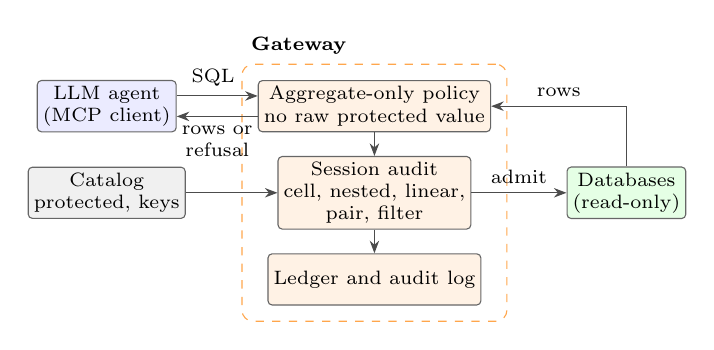
\begin{tikzpicture}[font=\scriptsize,
  box/.style={draw=black!60, rounded corners=1.5pt, fill=#1, minimum height=6.5mm, minimum width=23mm, align=center, inner sep=2pt},
  box/.default=white, side/.style={box=#1, minimum width=14mm},
  arr/.style={-{Stealth[length=1.6mm]}, draw=black!70}]
\node[box=orange!10] (enf) at (0,-1.1) {Aggregate-only policy\\no raw protected value};
\node[box=orange!10] (aud) at (0,-2.2) {Session audit\\cell, nested, linear,\\pair, filter};
\node[box=orange!10] (led) at (0,-3.3) {Ledger and audit log};
\node[draw=orange!70, dashed, rounded corners, fit=(enf)(aud)(led), inner sep=2mm] (gw) {};
\node[font=\scriptsize\bfseries, anchor=south west] at (gw.north west) {Gateway};
\node[side=blue!8] (agent) at (-3.4,-1.1) {LLM agent\\(MCP client)};
\node[side=green!10] (db) at (3.2,-2.2) {Databases\\(read-only)};
\node[side=gray!12] (cat) at (-3.4,-2.2) {Catalog\\protected, keys};
\draw[arr] ([yshift=1.3mm]agent.east) -- node[above, pos=0.45]{SQL} ([yshift=1.3mm]enf.west);
\draw[arr] ([yshift=-1.3mm]enf.west) -- node[below, pos=0.5, align=center]{rows or\\refusal} ([yshift=-1.3mm]agent.east);
\draw[arr] (enf) -- (aud);
\draw[arr] (aud) -- (led);
\draw[arr] (aud.east) -- node[above]{admit} (db.west);
\draw[arr] (db.north) |- node[pos=0.75, above]{rows} (enf.east);
\draw[arr] (cat.east) -- (aud.west);
\end{tikzpicture}
\caption{Gateway between LLM agents and databases. The policy check refuses a query that returns a protected column; the session audit refuses a query whose answer would rest on fewer than $k$ entities given earlier answers, using the ledger of entity sets behind admitted answers; only admitted queries reach the read-only connection.}
\label{fig:arch}
\end{figure}

\paragraph{Sessions} A session starts with a purpose, which names the protected columns, $k$, and the identity the session runs under. The gateway keeps two pieces of state for it: the ledger of entity sets behind admitted answers, per protected column, and the set of entities whose sensitive columns were returned raw, checked against the purpose's entity budget. A refused query changes neither, because nothing was released. Calling \texttt{begin\_session} again, with the same or another purpose, keeps the ledger, since it is keyed by protected column rather than by purpose; and the ledger is stored per authenticated identity, so a new connection under the same identity does not start from an empty ledger either.

\subsection{Aggregate-only policy}\label{sec:policy}
A purpose declares which columns are \emph{protected}. Like an aggregation policy in an analytical database, it allows a protected column inside SUM and AVG and refuses any query that returns it. These two are linear in the protected values, which is what the session audit models. A protected column inside any other aggregate is refused wherever it appears, including HAVING: MIN, MAX, MEDIAN, percentiles and list aggregates can return one entity's exact value, and VARIANCE and STDDEV release a second moment, so an average of 100 with a variance of 0 fixes every value in the group however large it is. The gateway classifies each use $o$ of a column $c$ in a query $q$ as \textsf{raw} if $o$ is returned (in the outer select list outside any aggregate, or the argument of a projected MIN or MAX), \textsf{agg} if $o$ is inside a value aggregate, and \textsf{filter} otherwise (WHERE, JOIN, GROUP BY, ORDER BY, or inside COUNT). Columns are resolved to $t.c$ by qualifying $q$ against the schema, so aliases, joins and subqueries are handled; a query that cannot be resolved is refused. A query that uses a protected column in mode \textsf{raw}, or a column outside the purpose, is refused before it runs.

\paragraph{Example} In Fig.~\ref{fig:example}a the balance is used in mode \textsf{agg} and the segment, nation key and customer key in mode \textsf{filter}, so both queries pass this rule. A query returning one customer's balance would not. The policy alone therefore stops direct reads but not the combination of two allowed averages; that is the job of the session audit.

\subsection{Session audit}\label{sec:audit}
The audit asks one question before each query runs: if this answer is released, how few people could it be about, given everything already released? It answers with entity sets. Let $p\in P$ be a protected column of entity table $E(p)$ with key $\kappa$. For an admitted query that aggregates $p$, the gateway rewrites it to select $\kappa$ and the grouping expressions, dropping aggregation, HAVING, ORDER and LIMIT, and runs the rewrite on the read-only connection. This yields $\mathcal{S}(q)=\{S_1,\dots,S_m\}$, one set per output group, and for each a weight vector $w_S$, where $w_S(i)$ is the number of rows entity $i$ contributes to the group. Joins repeat entities: a SUM of balances over \texttt{customer JOIN orders} is $\sum_i w_S(i)\,x_i$ with $w_S(i)$ the customer's order count; without joins every weight is 1. Five tests follow.

Table~\ref{tab:notation} collects the symbols used in the rest of this section.

\begin{table}[!t]
\caption{Notation.}
\label{tab:notation}
\centering\footnotesize
\begin{tabular}{@{}l@{\ \ }p{0.68\columnwidth}@{}}
\toprule
Symbol & Meaning\\
\midrule
$P$, $E(p)$ & Protected columns; entity table and key of $p$\\
$\mathcal{S}(q)$, $\mathcal{C}(q)$ & Entity sets of $q$'s groups; candidate sets of $q$'s protected filter\\
$\mathcal{H}$, $\mathcal{H}_{\downarrow}$ & Sets of earlier admitted aggregates and protected filters\\
$k$ & Minimum number of entities an answer may rest on\\
$w_S$, $Q$ & Weights of group $S$ (rows per entity); orthonormal basis of answered weights\\
\bottomrule
\end{tabular}
\end{table}

\emph{Small-cell test.} The first test asks how many entities the smallest group in the answer covers:
\begin{equation}\label{eq:cell}
\iota_1(q)=\min_{S\in\mathcal{S}(q)}|S|.
\end{equation}

\emph{Nested-pair test.} Take Fig.~\ref{fig:example}a. The first answer covers 12 customers and the second covers 11 of the same 12. Neither group is small, but exactly one customer is in the first and not the second, and subtracting the two sums gives that customer's balance. The nested-pair test finds every pair of answers in which one group contains the other and counts the entities in the difference. With $\mathcal{H}$ the groups of earlier admitted aggregates over $p$,
\begin{equation}\label{eq:pair}
\iota_2(q)=\min_{(A,B)\in N(q)}\bigl|\{i: w_B(i)>w_A(i)\}\bigr|,
\end{equation}
where $N(q)$ is the set of pairs from $\mathcal{S}(q)\cup\mathcal{H}$ with $w_A\le w_B$ entrywise and $w_A\ne w_B$, at least one of them in $\mathcal{S}(q)$. In Fig.~\ref{fig:example}a this count is 1, so for any $k\ge2$ the second query is refused.

\emph{Linear test.} Differences need not be nested: three overlapping groups, none containing another, can still be added and subtracted to leave one entity, and Section~\ref{sec:adaptive} shows attackers finding such combinations. The linear test therefore treats each answer as one equation in the unknown per-entity values and asks whether the equations admitted so far, together with the new one, can be solved for any single entity's value. A SUM answer is the inner product of $w_S$ with the vector of per-entity values; an AVG is the same once the group's COUNT is known. Entity $i$'s value is determined by the answers iff the unit vector $e_i$ lies in their span~\cite{chin1982auditing}. With $Q$ an orthonormal basis of $\{w_S:S\in\mathcal{H}\}$,
\begin{equation}\label{eq:linear}
e_i\in\operatorname{span}(Q)\iff (QQ^{\top})_{ii}=\textstyle\sum_j Q_{ij}^2=1,
\end{equation}
tested with tolerance $10^{-9}$ on normalized weight vectors, and the set of entities $q$ would newly disclose is $D(q)=\{i: (Q'Q'^{\top})_{ii}=1\}$, where $Q'$ extends $Q$ by Gram--Schmidt with $w_S$ for $S\in\mathcal{S}(q)$. The weights are taken only from the bare column: SUM or AVG of an expression of $p$ (a product, a CASE, DISTINCT) is not a weighted sum the audit can model, and is refused. One shape is the exception, because it is a filtered sum in disguise: a conditional aggregate such as \texttt{SUM(CASE WHEN} $c$ \texttt{THEN} $p$ \texttt{ELSE 0 END)} returns the same value as \texttt{SUM(}$p$\texttt{) WHERE} $c$. The gateway audits such a query as several queries: one filtered aggregate per conditional aggregate, plus the remainder with each conditional aggregate replaced by a constant. ORDER, LIMIT, HAVING and DISTINCT are dropped from each part, which can only enlarge its groups' exposure, never shrink it. The parts are checked in turn against the session state, and the query is admitted only if every part is; if one is refused, nothing from the earlier parts is kept.

\emph{Combination test.} The linear test stops one entity's value, but an attacker can settle for a combination of a few. Suppose customers $t$ and $u$ appear together in one group with three others, $R_1$, and the agent also asks for $R_1\cup R_2$ and for $R_2$ alone. No group is small, no nested pair differs by fewer than three customers, and neither $e_t$ nor $e_u$ lies in the span, yet the first answer minus the second plus the third is $x_t+x_u$. Swapping one customer for another in an otherwise equal group gives $x_t-x_u$ in the same way, and the same three queries with $m$ targets give the sum of their $m$ balances. The combination test refuses a query after which some linear function of fewer than $k$ entities' values would be determined. Such a function exists exactly when some set $T$ of fewer than $k$ entities is essential to the answers: deleting $T$'s entities from every group would lower the rank of the answered weights.

The test finds such sets through \emph{leverage} $L_i=\lVert Q_i\rVert^2$, the squared norm of row $i$ of $Q$; $L_i=1$ is the linear test's condition, and the leverages sum to the rank $r$. A combination supported on $T$ needs $\sum_{i\in T}L_i\ge1$, so $T$ contains an entity with $L_i\ge1/|T|$, and at most $|T|\,r$ entities qualify. For two entities the condition has a closed form,
\begin{equation}\label{eq:pairtest}
a\,e_i+b\,e_j\in\operatorname{span}(Q)\iff (1-L_i)(1-L_j)=(Q_i\cdot Q_j)^2 ,
\end{equation}
because the $2\times2$ block of $QQ^{\top}$ on $\{i,j\}$ must have eigenvalue 1; only entities with $L_i\ge\frac12$, at most $2r$ of them, need partners. For a combination of up to $s>2$ entities, the test takes each \emph{anchor} $i$ with $L_i\ge 1/s$, deletes coordinate $i$ from the span, and searches what remains for a combination of up to $s-1$ entities, ending in Eq.~\ref{eq:pairtest}. Deleting row $i$ keeps the basis orthonormal after a rank-one correction, $Q_{-i}\bigl(I+(1/\sqrt{1-L_i}-1)\,Q_i^{\top}Q_i/L_i\bigr)$, at cost $O(nr)$. Let $D_{<k}(q)$ be the sets of fewer than $k$ entities this search finds once $q$'s sets are added; for $k\le2$ it is empty, since the linear test already covers one entity.

\emph{Filter test.} A protected column can leak without being aggregated. In Fig.~\ref{fig:example}b the query counts rows, not balances, but the count is over one customer, so it is 0 or 1 according to whether that customer's balance passes the threshold. The filter test asks which entities' protected values the answer depends on, and applies the three tests above to those entities. When $q$ uses $p$ in its WHERE clause outside any aggregate, the gateway \emph{relaxes} $q$: it replaces every comparison on $p$ with TRUE, which yields a query $q^{\downarrow}$ that matches a superset of $q$'s rows. The candidate sets $\mathcal{C}(q)$ are the entity sets of $q^{\downarrow}$'s output groups, or one singleton per entity if $q$ returns rows rather than aggregates. The gateway applies Eqs.~\ref{eq:cell}--\ref{eq:pairtest} to $\mathcal{C}(q)$ against a separate history $\mathcal{H}_{\downarrow}$, giving $\iota_{\downarrow}(q)$ and $D_{\downarrow}(q)$. In Fig.~\ref{fig:example}b the relaxed query matches one customer, so its candidate set holds one entity and the first probe is refused.

Relaxation gives a superset only for comparisons joined by AND and OR, so a protected column under NOT or CASE, in JOIN ON, GROUP BY, ORDER BY or HAVING, or in a subquery, is refused. So is SUM, AVG, MIN or MAX of a non-protected column under such a filter: summing known, distinct order totals over the customers whose balance passes a threshold would decode which of them passed. Unequal weights decode it too (a \texttt{COUNT(*)} over a join where the target has three orders and two others one each shows whether the target passed), so every candidate in a group must carry the same weight unless the query is \texttt{COUNT(DISTINCT}~$\kappa$\texttt{)}.

The gateway refuses $q$ iff
\begin{equation}\label{eq:refuse}
\min(\iota_1(q),\iota_2(q),\iota_{\downarrow}(q))<k\,\text{or}\,D(q)\cup D_{\downarrow}(q)\cup D_{<k}(q)\cup D_{<k\downarrow}(q)\ne\emptyset .
\end{equation}
A refused query reveals nothing, so its sets enter no history. Eq.~\ref{eq:cell} alone is the stateless baseline (cell suppression); Eqs.~\ref{eq:cell}--\ref{eq:pair} form the pairwise audit; Eqs.~\ref{eq:cell}--\ref{eq:linear} the linear audit; Eq.~\ref{eq:refuse} in full adds the combination test.

\paragraph{Nested queries and fail-closed coverage} The gateway merges every CTE and derived table that only filters, joins or renames into the query that reads it. Each one left that reads a protected column, typically a total per group, is audited as an answer of its own before the query that reads it, and the query is admitted only if every part is. The final answer then depends on protected values only through admitted answers, so it reveals nothing beyond them, at the cost of refusing a total per person even when the final answer only averages it. A protected column that a CTE passes on outside an aggregate counts as returned. The gateway refuses what it cannot attribute: a protected or sensitive column inside a set operation or recursive CTE, the entity table referenced twice within one part, nested queries over protected columns in strict mode (a filter on a CTE's total would make decisions depend on protected values), and any query whose rewrite fails. A rewrite that matches no entity is admitted, since the answer covers no one.

\paragraph{Entity budget} Some purposes need individual records: a support agent helping one customer must see that customer's details. Such a purpose carries an entity budget. The gateway counts the distinct entities whose sensitive columns were returned raw in the session and refuses a query that would return them for more entities than the purpose allows.

\subsection{Guarantees}\label{sec:guarantees}
We state what the audit guarantees precisely; Table~\ref{tab:guarantees} summarizes it per SQL feature.

\begin{table}[!t]
\caption{Guarantee per SQL feature over a protected column $p$. All rows assume values fixed while a ledger lives; none covers values in non-protected columns or collusion across identities.}
\label{tab:guarantees}
\centering\scriptsize
\setlength{\tabcolsep}{2pt}
\begin{tabular}{@{}p{0.36\columnwidth}p{0.17\columnwidth}p{0.2\columnwidth}p{0.21\columnwidth}@{}}
\toprule
SQL feature & Released & Covered by & What remains\\
\midrule
SUM, AVG of $p$ (joins, CASE, nesting) & sums $Ax$ & Props.~\ref{prop:linear}, \ref{prop:pair} & intervals if values are bounded\\
$p$ in a filter or COUNT & counts over thresholds & tests, no proof & across thresholds; strict refuses\\
Refusals & who matches & strict: Prop.~\ref{prop:strict} & may leak if not strict\\
$p$ returned, or in MIN, MAX, MEDIAN, VARIANCE, STDDEV, other aggregates or an expression & -- & refused & --\\
Set operation, recursive CTE, failed rewrite & -- & refused & --\\
\bottomrule
\end{tabular}
\end{table}

\begin{proposition}\label{prop:linear}
Let $A\in\mathbb{N}^{m\times n}$ have the weight vectors of the $m$ admitted aggregate groups over a protected column as rows, and let each answer be the exact sum $Ax$ of the unknown per-entity values $x\in\mathbb{R}^n$. If no admitted query satisfied $D(q)\ne\emptyset$, then for every entity $i$ and every $x$ there is $x'$ with $Ax'=Ax$ and $x'_i\ne x_i$.
\end{proposition}
\begin{proof}
Each admission checked Eq.~\ref{eq:linear} with the query's sets added, so after the last admission $e_i\notin\operatorname{row}(A)$ for every $i$; refused queries add no rows. Since $\operatorname{row}(A)=\operatorname{null}(A)^{\perp}$, $e_i\notin\operatorname{row}(A)$ implies some $z\in\operatorname{null}(A)$ has $z_i\ne0$. Put $x'=x+z$. Then $Ax'=Ax$ and $x'_i=x_i+z_i\ne x_i$. The test itself is exact because $(QQ^{\top})_{ii}=\lVert QQ^{\top}e_i\rVert^2$ equals 1 iff $e_i$ lies in the span.
\end{proof}

\begin{proposition}\label{prop:pair}
Under the same conditions, if no admitted query satisfied $D_{<k}(q)\ne\emptyset$, then no nonzero linear function of the values of fewer than $k$ entities is determined by the answers.
\end{proposition}
\begin{proof}
As in Proposition~\ref{prop:linear}, $c^{\top}x$ is determined iff $c\in V=\operatorname{row}(A)=\operatorname{span}(Q)$. (a) If $c\in V$ has unit norm and support $T$, then $1=c^{\top}QQ^{\top}c\le\lambda_{\max}\bigl((QQ^{\top})_{TT}\bigr)\le\sum_{i\in T}L_i$, so some $i\in T$ has $L_i\ge1/|T|$ and is tried as an anchor. (b) Let $L_i<1$ and let $V_{-i}$ be $V$ with coordinate $i$ deleted. If $c\in V$ is supported on $T\ni i$, then $c_{-i}\in V_{-i}$ is nonzero (otherwise $e_i\in V$ and $L_i=1$) and supported on $T\setminus\{i\}$; conversely, a nonzero $d\in V_{-i}$ supported on $T'$ is $c_{-i}$ for some $c\in V$ supported on $T'\cup\{i\}$. So $V$ has a nonzero vector on at most $s$ entities through $i$ iff $V_{-i}$ has one on at most $s-1$. (c) $Q_{-i}^{\top}Q_{-i}=I-Q_i^{\top}Q_i$, whose inverse square root is the correction above, so the recursion works on an orthonormal basis of $V_{-i}$. Induction on $s$, with Eq.~\ref{eq:linear} and Eq.~\ref{eq:pairtest} as base cases, shows the search is exact. Refused queries add no rows.
\end{proof}

The search is exponential in $k$, and no algorithm can avoid that in general.

\begin{theorem}\label{thm:hard}
Given $A\in\mathbb{N}^{m\times n}$ and $k$, deciding whether some nonzero vector of $\operatorname{row}(A)$ is supported on fewer than $k$ entities is NP-complete.
\end{theorem}
\begin{proof}
It is in NP: a set $T$ is a certificate, checked by testing whether deleting the columns $T$ lowers the rank of $A$. For hardness we reduce from deciding whether a rational matrix $W\in\mathbb{Q}^{d\times n}$ has a circuit of at most $s<n$ columns, that is, a nonzero $z$ with $Wz=0$ and at most $s$ nonzero entries, which is NP-complete~\cite[Thm.~1]{tillmann2014complexity}. Compute a rational basis $N_1,\dots,N_t$ of $\operatorname{null}(W)$ and let $V\subseteq\mathbb{R}^{2n}$ be spanned by the vectors $(N_j,0)$ and the all-ones vector $\mathbf{1}$. Every vector of $V$ is $(z+\lambda\mathbf{1},\lambda\mathbf{1})$ with $Wz=0$; if $\lambda\ne0$ it has at least $n>s$ nonzero entries, and if $\lambda=0$ it is $(z,0)$. So $V$ has a nonzero vector on at most $s$ entries iff $W$ has a circuit of at most $s$ columns. The vectors $(N_j,0)+\mu\mathbf{1}$ for a large rational $\mu$, together with $\mathbf{1}$, are nonnegative and still span $V$; scaled by a common denominator they form $A$, of size polynomial in that of $W$. Set $k=s+1$.
\end{proof}

So no audit runs in time polynomial in both $n$ and $k$ unless P\,=\,NP. The search above is polynomial for each fixed $k$: level $s$ tries at most $s\,r$ anchors, so it runs at most $\frac{(k-1)!}{2}\,r^{k-3}$ pair searches (Eq.~\ref{eq:pairtest}), each $O(nr^2)$, with the exponent on the rank rather than on the number of entities. The reduction uses general nonnegative weights, as joins produce; whether the problem stays hard for plain sets, with every weight 0 or 1, we leave open.

The filter test has no such proof; exact filter auditing is hard even for Boolean values~\cite{kleinberg2003boolean}. A count under a threshold is linear in the indicator vector of that threshold, $[x_j>t]_j$, and different thresholds give different unknown vectors. The audit treats all filters on $p$ as one unknown, which refuses every single-entity probe and every nested or linear combination of candidate sets, but an attacker who combines answers across thresholds is not covered by Proposition~\ref{prop:linear}. Strict mode closes that gap.

\paragraph{Strict mode} Refusals can leak too: the decision depends on which entities match a query, and if membership depends on protected values, a refusal says something about them~\cite{kenthapadi2005simulatable}. In strict mode the gateway refuses any query that uses a protected column outside an aggregate.

\begin{proposition}\label{prop:strict}
In strict mode, the sequence of gateway decisions for a session is a function of the queries and of the non-protected columns only.
\end{proposition}
\begin{proof}
The aggregate-only policy and the strict check depend only on the query text. For an admitted aggregate, the key-only rewrite reads no protected column; the entity sets $\mathcal{S}(q)$ and their weights, and hence Eqs.~\ref{eq:cell}--\ref{eq:refuse}, depend only on non-protected data. By induction over the session, $\mathcal{H}$ and $Q$ do too.
\end{proof}

\subsection{Per-query procedure}\label{sec:pipeline}
Algorithm~\ref{alg:gateway} puts the policy check and the session audit together in the order the gateway applies them.

\begin{algorithm}[!t]
\caption{Gateway check for query $q$ under a purpose}\label{alg:gateway}
\begin{algorithmic}[1]
\State resolve every column of $q$ to $t.c$; \textbf{if} unresolvable \textbf{return} refuse
\State \textbf{if} $q$ touches a protected or sensitive column inside a set operation or recursive CTE \textbf{return} refuse
\State merge CTEs and derived tables that only filter or rename; split the rest into parts, each CTE over a protected column first and $q$ last; check each part in turn, and keep none if one is refused \Comment{Sec.~\ref{sec:audit}}
\State \textbf{if} $q$ returns a protected column, uses one in a non-linear aggregate, or uses a column outside the purpose \textbf{return} refuse \Comment{Sec.~\ref{sec:policy}}
\State \textbf{if} strict and $q$ filters on a protected column \textbf{return} refuse
\State split conditional aggregates into parts; check each part in turn, and keep none if one is refused
\For{$p\in P$ used by $q$ in a filter}
  \State $\mathcal{C}\gets$ candidate sets of the relaxed rewrite; \textbf{if} it fails \textbf{return} refuse
  \If{$\iota_{\downarrow}<k$ \textbf{or} $D_{\downarrow}(q)\cup D_{<k\downarrow}(q)\ne\emptyset$} \Return refuse \Comment{Eq.~\ref{eq:refuse}} \EndIf
\EndFor
\For{$p\in P$ used by $q$ in mode \textsf{agg}}
  \State $\mathcal{S}\gets$ entity sets of the key-only rewrite; \textbf{if} it fails \textbf{return} refuse
  \State \textbf{if} more groups than the limit \textbf{return} refuse
  \If{$\min(\iota_1,\iota_2)<k$ \textbf{or} $D(q)\cup D_{<k}(q)\ne\emptyset$} \Return refuse \Comment{Eq.~\ref{eq:refuse}} \EndIf
\EndFor
\State \textbf{if} sensitive columns returned raw for more entities than the budget \textbf{return} refuse
\State commit $\mathcal{S}$, $\mathcal{C}$ to $\mathcal{H}$, $\mathcal{H}_{\downarrow}$ and their bases; save the ledger; execute $q$; log
\State \Return rows
\end{algorithmic}
\end{algorithm}

\subsection{Cost}
Parsing and qualification are linear in the query size. Each rewrite costs one extra query whose result size is the number of matching rows. The linear test keeps $Q\in\mathbb{R}^{n\times r}$ over the $n$ entities touched so far and rank $r\le n$; adding a set costs $O(nr)$ with two Gram--Schmidt passes for stability, and Eq.~\ref{eq:linear} costs $O(nr)$. A query with more groups than a configurable limit (2,000 in our runs) is refused rather than audited. Table~\ref{tab:scaling} measures the check: \Nscalesmallms{} ms with 1,000 entities and rank 10, and \Nscalebigms{} ms with 50,000 entities and rank 500, where the dense basis takes \Nscalebigmb{} MB. With 1,000,000 entities a check takes \Nscalemmidms{} ms at rank 100, but \Nscalemms{} s at rank \Nscalemrank, where the \Nscalemmb{} MB basis strains a 16 GB machine; the dense basis is the limit at that size. In the finance sessions the basis reaches a median rank of \Nrankmed{} (at most \Nrankmax) by the end of a session. At $k=3$ the combination test examines at most $2r$ high-leverage entities against their candidates and raised the median check from \Nlinmed{} to \Npairmed{} ms (Section~\ref{sec:attacker}); Section~\ref{sec:attacker} also measures $k=4$ and $5$.

\begin{table}[!t]
\caption{Linear-audit check time (median of 5) and basis memory vs.\ entities $n$ and rank $r$, for random contiguous key-range sets (Python/NumPy, Apple M-series CPU, single process).}
\label{tab:scaling}
\centering\footnotesize
\begin{tabular}{@{}rrrr@{}}
\toprule
$n$ & $r$ & Check (ms) & Basis (MB)\\
\midrule
\tabinput{tables/scaling.tex}
\tabinput{tables/scaling_1m.tex}
\bottomrule
\end{tabular}
\end{table}

% ─────────────────────────────────────────────────────────────────────────────
\section{Evaluation}\label{sec:eval}

The evaluation asks five questions, one per subsection: whether a per-query minimum group size suffices (RQ1), what each test prevents and costs (RQ2), whether the audit holds against adaptive and rule-aware attackers (RQ3), whether alarms or noise would do instead (RQ4), and what it costs in practice (RQ5).

\subsection{Setup}\label{sec:evalmethod}
\paragraph{Environment} Python~3.14, sqlglot~30.23 for parsing and qualification, SQLite and PostgreSQL~16, NumPy, and the MCP Python SDK~2.x. LLMs: gpt-4o-mini and gpt-4o through the OpenAI chat API (temperature 0.7 with a per-episode seed) as attackers, gpt-4o-mini also as an agent, and Claude Sonnet 5.5 through the Anthropic API as an agent on Spider~2.0 (it declined the attacker role in every episode). All prompts, model outputs and seeds are cached in the repository.

\paragraph{Data} \emph{PostgreSQL at scale.} TPC-H at scale factor~1 (150,000 customers) on PostgreSQL~16, with 200 random target customers and three benign workload mixes of 1,600 queries each.
\emph{TPC-H sessions.} A seeded TPC-H-shaped SQLite database (1,500 customers, 7,500 orders, synthetic values) has four purposes and a session generator: \Nnbenign{} benign analyst sessions (400 per purpose) with realistic noise (30\% contain one query outside the purpose's columns; finance sessions include drill-downs and overlapping histogram bands) and \Nnattack{} attack sessions in five families (drift, small cell, two-query differencing, three-query differencing, enumeration; the figures call differencing ``tracker''). Every session has 6--16 queries regardless of label, so length carries no label information.
\emph{BIRD sessions.} The human-written gold queries of BIRD's~\cite{li2023bird} \texttt{financial} (\Nfinnq{} queries) and \texttt{debit\_card\_specializing} (\Ndebitnq{}) databases are arranged into 200 random sessions of 6--16 queries per database.

\paragraph{Adaptive attackers} Each attacker is an LLM told it is red-teaming a privacy gateway over synthetic data and given one customer key; it must find that customer's exact balance in at most 15 queries, seeing rows or refusal reasons after each.

\paragraph{Baselines} The audit is compared in five modes: the small-cell test alone (\emph{stateless}); the small-cell and nested-pair tests (\emph{pairwise}); the small-cell, nested-pair, linear and filter tests (\emph{linear}); the linear audit with no filter on protected columns (\emph{strict}); and the linear audit with the combination test (\emph{final gateway}). For comparison with intent-level monitoring we also compute session scores: drift, the sensitivity-weighted number of distinct columns used outside the purpose; cell, $1/\min(\iota_1,\iota_2)$ over the session; and breadth, the number of distinct entities whose protected or sensitive columns were returned raw, divided by the purpose's entity budget.

\paragraph{Metrics} An attack session is \emph{prevented} if the gateway refuses its disclosing query or an earlier one. A benign query is a \emph{false refusal} if the gateway refuses it. In the adaptive study a target is \emph{disclosed} if the answers the gateway returned determine its value exactly, as an oracle applying Eq.~\ref{eq:linear} decides, whatever the attacker claims.

\paragraph{Statistical reporting} For a proportion we report the 95\% Wilson score interval. Session-alarm thresholds are set per purpose on a held-out half of the benign sessions; detection rates are measured on the other half plus all attacks.

\subsection{RQ1: Does a per-query minimum group size suffice?}\label{sec:gap}
It does not: a minimum group size stops attacks that aggregate over few people, but differencing attacks recovered every target's exact balance, on PostgreSQL and against the aggregation controls of Snowflake and BigQuery, while the session audit stopped every attack.

We ran five attacks against 200 random target customers on PostgreSQL~16 at TPC-H scale factor~1, under three defenses: a broad reporting role with no aggregate rule, a per-query minimum group size of $k=3$ that counts distinct customers, and the gateway. Table~\ref{tab:gap} gives the results. The minimum group size refuses the AVG over one customer, the cell of one customer and every probe of the COUNT bisection, because each query rests on one customer. It admits both differencing attacks for all 200 targets, because each of their queries covers many customers. The session audit refuses all five.

\paragraph{On Snowflake and BigQuery} Both vendors' controls, set to a minimum of $\Nsnowflakek$ customers (last four columns of Table~\ref{tab:gap}), stopped the single-customer AVG and the COUNT bisection: they suppress a too-small group, measured after the filter. BigQuery forbids comparisons on its privacy unit column, the customer key, so its attacker selects customers by name instead. Both admitted every differencing attack and a bisection that also counts 50 further customers unconditionally, which keeps every group large while the count still moves with the target's balance. On each, \Nsnowflakebypass{} attacks recovered every target; with the gateway in front, none did.

On three benign workload mixes the two controls refuse the same share of queries. These mixes run at scale factor~1, where groups hold hundreds of customers; on the smaller finance sessions of Section~\ref{sec:prevent}, where drill-downs differ by only a few customers, the session tests raise benign refusals from \Nrefkthreestateless\% to \Nrefkthreelinear\%, mostly in sessions that genuinely isolate one customer.

\begin{table}[!t]
\caption{Per-query minimum group size vs.\ the session audit on PostgreSQL~16 (TPC-H scale factor~1), and each vendor's own control alone and behind the gateway (\emph{+audit}) on Snowflake and BigQuery. Upper part: targets whose exact balance the attack recovered (bold: none). Lower part: benign queries refused in three workload mixes (mostly large groups / balanced / drill-down heavy; 1,600 each). \emph{Min-group}: a per-query minimum of $k=3$ customers with no memory.}
\label{tab:gap}
\centering\scriptsize
\setlength{\tabcolsep}{2.4pt}
\begin{tabular}{@{}lccccccc@{}}
\toprule
& \multicolumn{3}{c}{PostgreSQL} & \multicolumn{2}{c}{Snowflake} & \multicolumn{2}{c}{BigQuery}\\
\cmidrule(lr){2-4}\cmidrule(lr){5-6}\cmidrule(lr){7-8}
Attack & Broad & Min-group & Audit & Alone & +audit & Alone & +audit\\
\midrule
\tabinput{tables/gap.tex}
\bottomrule
\end{tabular}
\end{table}

\subsection{RQ2: What does each test prevent, and at what cost?}\label{sec:prevent}
The linear audit prevents every scripted differencing attack at the same benign cost as the weaker pairwise audit.

The audit refuses only the query that would complete an isolation (Eq.~\ref{eq:refuse}). Table~\ref{tab:modes} compares the four modes at $k=3$ on the finance sessions, and Fig.~\ref{fig:audit} adds $k=2$ and $k=5$. The small-cell test alone stops almost no differencing. The pairwise audit stops two-query attacks but only \Nprevkthreepairwisetrackerthree\% of three-query attacks, whose sets are not nested. The linear audit stops both and refuses \Nrefkthreelinear\% of benign queries, the same as the pairwise audit: honest workloads rarely produce exact linear dependencies that the small-cell and nested-pair tests do not already catch.

Strict mode keeps the same protection but refuses \Nrefkthreestrict\% of benign queries, because analysts filter on balances (histogram bands, drill-downs above a threshold). At $k=5$ every non-strict mode refuses \Nrefkfivelinear\% of benign queries, because ordinary nation-by-segment groupings contain fewer than five customers.

\begin{table}[!t]
\caption{Audit modes at $k=3$ on the finance sessions. \emph{Prevented}: attack sessions refused at or before the disclosing query, for two-query and three-query differencing. \emph{Refused}: benign queries refused. \emph{Sessions}: benign sessions with at least one refusal.}
\label{tab:modes}
\centering\footnotesize
\setlength{\tabcolsep}{4pt}
\begin{tabular}{@{}lcccc@{}}
\toprule
 & \multicolumn{2}{c}{Prevented} & \multicolumn{2}{c}{Benign cost}\\
Mode & Two-query & Three-query & Refused & Sessions\\
\midrule
Stateless & \Nprevkthreestatelesstracker\% & \Nprevkthreestatelesstrackerthree\% & \Nrefkthreestateless\% & \Nhitkthreestateless\%\\
Pairwise & \Nprevkthreepairwisetracker\% & \Nprevkthreepairwisetrackerthree\% & \Nrefkthreepairwise\% & \Nhitkthreepairwise\%\\
Linear & \Nprevkthreelineartracker\% & \Nprevkthreelineartrackerthree\% & \Nrefkthreelinear\% & \Nhitkthreelinear\%\\
Strict & \Nprevkthreestricttracker\% & \Nprevkthreestricttrackerthree\% & \Nrefkthreestrict\% & \Nhitkthreestrict\%\\
\bottomrule
\end{tabular}
\end{table}

\begin{figure}[!t]
\centering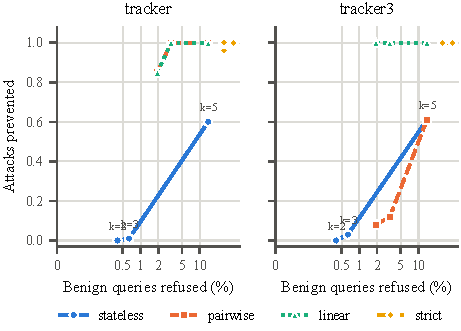
\includegraphics[width=0.85\columnwidth]{figures/fig7_audit_tradeoff.pdf}
\caption{Query-level audit on finance sessions: share of attacks prevented vs.\ share of benign queries refused, for $k\in\{2,3,5\}$ and the four audit modes. Left: two-query differencing; right: three-query differencing whose sets are not nested. $x$ axis symmetric-log.}
\label{fig:audit}
\end{figure}

\paragraph{Filter test and join weights}\label{sec:probes}
Both are needed: each of the two scripted probes below succeeds when the corresponding rule is removed and fails when it is applied.

\emph{Threshold probing.} Without the filter test, 21 counts of the form \texttt{COUNT(*) WHERE c\_custkey = 570 AND c\_acctbal > $t$} recovered the target's balance to the cent with no refusal. With the filter test the first probe is refused, since its candidate set holds one customer.

\emph{Join fan-out.} Without the weights, two probes succeed. Sixteen admitted SUMs over \texttt{customer JOIN orders} in date windows where customers have different order counts, plus those counts, determined customer 570's balance within 227 queries; a \texttt{COUNT(*)} bisection over a window where the target has three orders and two others one each recovered it in 21 probes. With weights, the first attack leaves the value undetermined after 1{,}192 queries (334 refused); the equal-weight rule refuses the second at its first probe.

\subsection{RQ3: Does it hold against attackers that adapt or know its rules?}\label{sec:adaptive}
For exact disclosure it does: under the linear audit no adaptive LLM attacker disclosed a target, while every weaker defense was defeated, and an attacker that knows the rules is stopped once the combination test is added.

We ran \Nadvnm{} targets per defense with gpt-4o-mini and \Nadvno{} with gpt-4o; gpt-4o was run in strict mode only against the final gateway. Fig.~\ref{fig:adaptive} and Table~\ref{tab:adaptive} report disclosure as decided by the oracle.

Every defense weaker than the linear audit was defeated. With the aggregate-only rule alone, both attackers succeed almost always, usually with one AVG over a single key. The stateless audit stops direct isolation but not differencing. The pairwise audit is defeated by combinations it does not model, such as overlapping key ranges. It was defeated more often than the stateless audit, though not significantly (Fisher's exact test, $p=\Nfisherm$ and $\Nfishero$).

Under the linear audit no target was disclosed by either attacker: 0 of \Nadvnm{} and 0 of \Nadvno{}, with upper 95\% bounds of \Nadvmlinearhi\% and \Nadvolinearhi\%. Strict mode gives \Nadvmstrict\% disclosure for gpt-4o-mini, with refusals that by Proposition~\ref{prop:strict} carry no information about balances.

We then ran both attackers against the final gateway, with and without strict mode, on the same targets. No target was disclosed (upper 95\% bounds \Nfinmlphi\% and \Nfinolphi\%), and no answer set determined any combination of the target with one other customer, which is what the combination test protects at $k=3$. The attackers met more refusals (\Nfinmlpref{} per gpt-4o-mini episode) and none stopped early with a correct answer.

\begin{table}[!t]
\caption{Adaptive LLM attackers. Upper part: an ablation that adds one test at a time, run without the filter test or fail-closed handling. Lower part: the final gateway of Section~\ref{sec:method}, with the combination test, filter test and fail-closed handling. \emph{Disclosed}: share of targets whose exact balance the returned answers determine. \emph{Refusals}: mean refusals per episode. Each pair is gpt-4o-mini (\Nadvnm{} targets) / gpt-4o (\Nadvno{} targets).}
\label{tab:adaptive}
\centering\footnotesize
\begin{tabular}{@{}lcc@{}}
\toprule
Defense & Disclosed & Refusals\\
\midrule
Aggregate-only rule & \Nadvmpurpose\% / \Nadvopurpose\% & \Nadvmpurposerefusals{} / \Nadvopurposerefusals\\
Stateless audit & \Nadvmstateless\% / \Nadvostateless\% & \Nadvmstatelessrefusals{} / \Nadvostatelessrefusals\\
Pairwise audit & \Nadvmpairwise\% / \Nadvopairwise\% & \Nadvmpairwiserefusals{} / \Nadvopairwiserefusals\\
Linear audit & \Nadvmlinear\% / \Nadvolinear\% & \Nadvmlinearrefusals{} / \Nadvolinearrefusals\\
Strict mode & \Nadvmstrict\% / -- & \Nadvmstrictrefusals{} / --\\
\midrule
Final gateway & \Nfinmlpdisc\% / \Nfinolpdisc\% & \Nfinmlpref{} / \Nfinolpref\\
Final gateway, strict & \Nfinmspdisc\% / \Nfinospdisc\% & \Nfinmspref{} / \Nfinospref\\
\bottomrule
\end{tabular}
\end{table}

\begin{figure}[!t]
\centering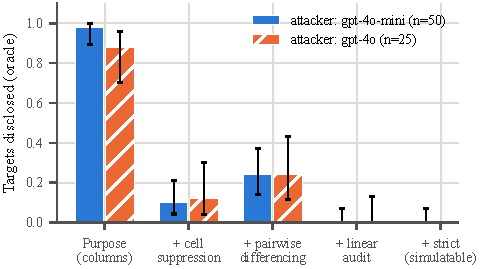
\includegraphics[width=0.85\columnwidth]{figures/fig8_adaptive_attacker.pdf}
\caption{Adaptive LLM attackers: share of targets whose exact balance is determined by the answers the gateway returned (oracle, Eq.~\ref{eq:linear}), per defense and attacker model. Bars: 95\% Wilson intervals.}
\label{fig:adaptive}
\end{figure}

\paragraph{An attacker that knows the rules}\label{sec:attacker}
Without the combination test it does not: a programmatic attacker recovered sums and differences of two customers' balances for every target, and exact balances through threshold counts. With the combination test every attack failed, and no benign query was refused that the linear audit admitted.

The LLM attackers do not know how the audit decides. We wrote an attacker that does and aims at the gaps Section~\ref{sec:guarantees} leaves: the two-customer sum and difference of Section~\ref{sec:audit}, and threshold counts on two overlapping groups $\{t,a,b\}$ and $\{a,b,c\}$. The third attack bisects \texttt{COUNT(*)} at each rank to recover the sorted balances of each group, about \Nprogthreshq{} queries per target, and takes the multiset difference, which is $x_t$. Each attack ran on \Nprogn{} random targets (\Nprognthresh{} for the third) on the TPC-H sessions' database at $k=3$. Table~\ref{tab:attacker} gives the results. Strict mode stops the threshold attack, since it refuses every filter on balances, but not the other two, which use only sums. The combination test stops all three: the first two because their answers determine $x_t+x_u$ or $x_t-x_u$, and the third because the two candidate sets differ by two customers. On the finance sessions it refused no further benign query.

\begin{table}[!t]
\caption{Programmatic attacker that knows the audit's rules, $k=3$: targets whose value the attack recovered exactly (sum or difference for the first two rows, the balance itself for the third; bold: none). Lower part: cost on the benign finance sessions.}
\label{tab:attacker}
\centering\scriptsize
\setlength{\tabcolsep}{3pt}
\begin{tabular}{@{}lccc@{}}
\toprule
Attack & Linear & Strict & Linear + combination\\
\midrule
\tabinput{tables/attacker.tex}
\bottomrule
\end{tabular}
\end{table}

Larger $k$ asks the combination test to look further. The same three queries with $m$ targets, padded with groups of $k$ customers so that the small-cell test admits them, reveal the sum of $m$ balances; it must be refused when $m<k$. Table~\ref{tab:support} runs this attack on \Nsupn{} target sets for $k=3,4,5$ and $m=2,3,4$. Checking pairs only, as Eq.~\ref{eq:pairtest} does, misses the three- and four-customer sums at $k=4$ and $5$; the full combination test refuses every attack with $m<k$ and admits every one with $m\ge k$, which rests on enough customers. On the benign finance sessions it refused no query that the linear audit admitted: \Nsupfourcombref\% and \Nsupfivecombref\% of queries at $k=4$ and $5$, the same as the linear audit alone, where the higher rate at $k=5$ comes from the small-cell test. The median check stayed at \Nsupfourcombmed{} and \Nsupfivecombmed{} ms.

\begin{table}[!t]
\caption{Sum of $m$ customers' balances from three padded SUMs, at minimum size $k$: target sets recovered out of \Nsupn{}, checking pairs only / with the full combination test (bold: none). Right: benign finance queries refused (pairs / full) and check time of the full test.}
\label{tab:support}
\centering\scriptsize
\setlength{\tabcolsep}{2.5pt}
\begin{tabular}{@{}lccccc@{}}
\toprule
$k$ & $m=2$ & $m=3$ & $m=4$ & Refused (\%) & ms (med / 95th)\\
\midrule
\tabinput{tables/support.tex}
\bottomrule
\end{tabular}
\end{table}

\subsection{RQ4: Would alarms or noise do instead?}\label{sec:alarms}
Neither would. Session signals separate the attacks that show in the shape of a session, and they miss differencing, because honest sessions produce the same pattern.

We computed the AUROC of every signal for every attack family against held-out benign sessions of the same purpose. Session length carries no label information (query-count AUROC \Naucdriftqueries--\Naucenumerationqueries). Three families are separated almost perfectly by the signal that measures their mechanism: drift by use of columns outside the purpose, enumeration by breadth, and small cells by the per-query cell test.

At a 1\% benign false-positive rate, session state helps where the violation is cumulative: drift detection rises from \Ntprstatelessordrift\% to \Ntprstatefulordrift\%, and enumeration detection from \Ntprstatelessorenumeration\% to \Ntprstatefulorenumeration\%.

For the aggregate families, session alarms detect almost nothing at this rate, because \Nbenignleak\% of benign finance sessions (\Nbenignleakn{} of \Nnfinbenign) genuinely isolate one customer, typically with an average by nation and segment followed by the same average restricted to positive balances, the pattern of Fig.~\ref{fig:example}a. The right tool refuses the single query that completes the isolation, as the audit does (Section~\ref{sec:prevent}).



\paragraph{Noise instead of refusal}\label{sec:dp}
On groups of about a dozen customers, none of the budgets we tried with the Laplace mechanism gave both useful answers and protection, while the audit returns exact answers and refuses a few queries.

Instead of refusing, a gateway could answer every aggregate with Laplace noise~\cite{dwork2006calibrating,johnson2018flex}. We clip balances to $[-1{,}000,10{,}000]$ (sensitivity 10,000 per SUM), split a session budget $\varepsilon$ equally across its protected aggregates, and answer an average as a noisy sum over the exact group size. Table~\ref{tab:dp} compares utility on the benign finance sessions with the share of differencing sessions in which the attacker's estimate lands within 10\% of the target's balance.

In this workload no budget we tried gives both. At $\varepsilon=10$ only \Ndptenfive\% of benign answers are within 5\% of the true value. At $\varepsilon=100$ most are, but the attacker then succeeds in \Ndphundredatt\% of sessions. The audit instead refuses \Nrefkthreelinear\% of benign queries and returns the rest exactly.

The comparison is narrow: it covers one mechanism, one clipping range and small groups, and does not show that differential privacy cannot serve such workloads, nor that the audit gives equivalent protection. Differential privacy bounds inference for every query and needs no entity sets, while the audit's guarantee covers exact disclosure through sums only (Table~\ref{tab:guarantees}). Differential privacy suits large groups and approximate dashboards; the audit suits exact answers over small groups.

\begin{table}[!t]
\caption{Differential privacy vs.\ the session audit on the finance workload. \emph{Median error}, \emph{Within 5\%}: relative error of benign answers per output group. \emph{Refused}: benign queries refused. \emph{Attacker}: share of differencing sessions whose estimate is within 10\% of the target's balance (audit: midpoint of the linear-programming bound; guessing the domain midpoint scores \Ndpauditprior\%).}
\label{tab:dp}
\centering\footnotesize
\setlength{\tabcolsep}{3.5pt}
\begin{tabular}{@{}lcccc@{}}
\toprule
Answering & Median error & Within 5\% & Refused & Attacker\\
\midrule
\tabinput{tables/dp.tex}
Linear audit, $k=3$ & 0\% & 100\% & \Nrefkthreelinear\% & \Ndpauditatt\%\\
\bottomrule
\end{tabular}
\end{table}

\subsection{RQ5: What does it cost on human-written queries and in deployment?}\label{sec:bird}
Little on short questions, more on long analytical ones. On human-written queries the audit costs only its per-query rules: the stateful tests refused nothing more, and the median check takes under a millisecond. LLM agents answering the same questions through the gateway lost no significant accuracy on questions it admits, while their correct answers to questions about one customer fell to zero. On longer Spider~2.0 tasks a stronger agent solved a quarter fewer behind the gateway, because those tasks take ratios, clamps or rankings of totals over one or a few people.

Here we replace the generated workloads with BIRD's human-written queries, under an analytics purpose that permits every column except per-entity amounts and balances, which may only be aggregated. Fig.~\ref{fig:bird} and Table~\ref{tab:bird} report the results.

The linear audit refuses \Nfinreflinear\% of queries on \texttt{financial} and \Ndebitreflinear\% on \texttt{debit\_card\_specializing}, and in both databases the stateless audit refuses the same share. The higher rate on the debit-card database reflects its questions, many of which ask for one customer's consumption; under an aggregate-only purpose those are disclosures by design, so the rate measures policy fit, not audit error.

To see why queries are refused, we ran each one alone in a fresh session (lower part of Table~\ref{tab:bird}). Most refusals come from the filter test. To judge whether the remaining refusals are errors, we classified each of the \Nbirdrefn{} queries refused alone from its question text. \Nbirddesign{} ask for one entity's value, for the top or bottom entity, or look up an exact amount to identify someone; under an aggregate-only purpose these are disclosures by design. \Nbirdfp{} are false positives, mostly counts over a join that the equal-weight rule refuses, and \Nbirdborder{} are borderline, such as revenue per gas station where some stations have few customers. The combination test leaves both refusal rates unchanged.

\begin{table}[!t]
\caption{Human-written BIRD workloads under the analytics purpose, $k=3$. Upper: sessions of 6--16 queries. Lower: each query alone in a fresh session, with the reason for refusal (reasons shown without the conditional split).}
\label{tab:bird}
\centering\footnotesize
\setlength{\tabcolsep}{4pt}
\begin{tabular}{@{}lcc@{}}
\toprule
 & \texttt{financial} & \texttt{debit\_card}\\
\midrule
Queries & \Nfinnq & \Ndebitnq\\
Refused: raw protected value & \Nfinmode\% & \Ndebitmode\%\\
Refused: stateless audit & \Nfinrefstateless\% & \Ndebitrefstateless\%\\
Refused: linear audit & \Nfinreflinear\% & \Ndebitreflinear\%\\
\quad with conditional split & \Nfinrefsplit\% & \Ndebitrefsplit\%\\
Refused: strict mode & \Nfinrefstrict\% & \Ndebitrefstrict\%\\
Entity sets computed & \Nfincovfinal\% & \Ndebitcovfinal\%\\
Check time, ms (median / 95th) & \Nfinlatmed{} / \Nfinlatp & \Ndebitlatmed{} / \Ndebitlatp\\
Query time, ms (median / 95th) & \Nfinqmed{} / \Nfinqp & \Ndebitqmed{} / \Ndebitqp\\
\midrule
Queries refused alone & \Nfinsingle & \Ndebitsingle\\
\quad without the filter test & \Nfinsingleold & \Ndebitsingleold\\
\quad with conditional split & \Nfinsinglesplit & \Ndebitsinglesplit\\
\quad Ranks or groups by protected value & \Nfincatrank & \Ndebitcatrank\\
\quad Filter depends on too few entities & \Nfincatthreshold & \Ndebitcatthreshold\\
\quad Aggregate under a protected filter & \Nfincatweighted & \Ndebitcatweighted\\
\quad Filtered count over a join & \Nfincatfanout & \Ndebitcatfanout\\
\quad Aggregate of an expression & \Nfincatexpression & \Ndebitcatexpression\\
\quad Aggregate over too few entities & \Nfincataggregate & \Ndebitcataggregate\\
\quad Shape cannot be audited & \Nfincatopaque & \Ndebitcatopaque\\
\bottomrule
\end{tabular}
\end{table}

\paragraph{Agents doing the tasks} An agent that is refused can rephrase, so we gave \Nagmodel{} each BIRD question with its schema and hint, let it run up to \Nagturns{} queries and see rows or the gateway's refusal reason, and scored its final query by BIRD's execution accuracy (same result set as the gold query). Table~\ref{tab:agent} compares an open read-only database with the gateway, each with and without the gateway's rules stated in the prompt, and the gateway with questions grouped into sessions of 6--16. We report the \Nagadmn{} questions whose gold query the gateway admits alone and the \Nagonen{} that ask for one entity's value (classified as above), and test paired differences with an exact McNemar test.

Without the rules in the prompt, the gateway did not significantly lower accuracy on admitted questions (\Naggatenradmfrom\% to \Naggatenradmto\%, $p=\Naggatenradmp$), while correct answers to one-entity questions fell to \Naggatenroneto\%, as intended (Table~\ref{tab:agent}). Stating the rules in the prompt cost more than the gateway did: it lowered accuracy on admitted questions even with no gateway at all ($p=\Nagpromptadmp$). We have not established why. Its one correct one-entity answer used a loan date that only one loan has and released no protected value. Grouping questions into sessions changed nothing.

\paragraph{Enterprise-style tasks} Spider~2.0~\cite{lei2024spider2} has longer analytical tasks over real schemas. On the \Nspn{} tasks of its SQLite subset whose databases hold per-person money or grades, we protected those columns and ran the same conditions, scored by Spider~2.0's comparison. \Nagmodel{} solved too few to show a cost (\Nspothopenc{} of the \Nspothn{} tasks that ask for no individual's value, with open access), so we also ran Claude Sonnet~5.5 (effort \emph{medium}), a stronger SQL agent that solved \Nssothopenc{} of them. Behind the gateway it solved \Nsnothgatec{} ($p=\Nsngatenrothp$). Each of the \Nsnlost{} tasks it still lost computes totals over one person or a few at some step and then applies a non-linear step to them: a growth rate or a share of lifetime sales, a balance clamped at zero, or a ranking that picks the cities with the lowest totals, which hold single orders. Such steps are not sums of the protected values, so the linear audit cannot admit them. Of the \Nsnentn{} tasks that ask for individuals' values, it solved \Nsnentopenc{} with open access and \Nsnentgatec{} behind the gateway. Both of those compute each customer's spending from invoice line prices, a column our purpose did not protect, so they show a gap in the column list rather than in the audit.

\begin{table}[!t]
\caption{LLM agents (\Nagmodel, up to \Nagturns{} queries) answering BIRD questions: execution accuracy (\%) by condition. \emph{Admitted}: gold query admitted alone. \emph{One-entity}: asks for one entity's value. Rules: stated in the prompt.}
\label{tab:agent}
\centering\scriptsize
\setlength{\tabcolsep}{2.5pt}
\begin{tabular}{@{}lccccc@{}}
\toprule
 & Open & \makecell{Open,\\rules} & \makecell{Gateway,\\rules} & Gateway & \makecell{Gateway,\\sessions}\\
\midrule
\tabinput{tables/agent.tex}
\bottomrule
\end{tabular}
\end{table}

\begin{figure}[!t]
\centering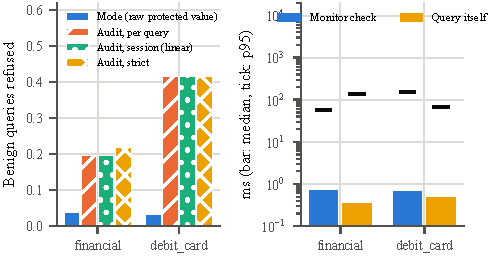
\includegraphics[width=0.85\columnwidth]{figures/fig9_bird_benign.pdf}
\caption{Human-written BIRD workloads (200 sessions per database). Left: share of benign queries refused. Right: monitor check time vs.\ query execution time (bars: median; ticks: 95th percentile; log scale).}
\label{fig:bird}
\end{figure}

\paragraph{Deployment over MCP}\label{sec:e2e}
Both deployment paths reproduced the library's decision on every query with 150,000 and with 1,000,000 customers, with a median check under five milliseconds; the cost is in the tail, which grows with the number of customers.

We loaded the TPC-H-shaped schema into PostgreSQL~16 at scale factor 1, generated \Neesessions{} benign and attack sessions (\Neequeries{} queries), and replayed them through two deployment paths: the gateway executing on Postgres itself, and the gateway forwarding to a separate database MCP server. Every attack in all five families was refused at or before its disclosing query. The median check took \Needirchkmed{} ms against a median query execution of \Needirexmed{} ms. We replayed the same sessions on a load with 1,000,000 customers and 10,000,000 orders. Decisions still matched the library on every query and every attack was refused, and the median check stayed at \Neemchkmed{} ms. The tail is the deployment bottleneck: on the direct path \Neemoverone{} of \Neemn{} checks took over a second, \Neemoverten{} over ten seconds and the slowest \Neemmax{}~s. All of them came from the finance purpose, and \Neemslowwhole{} were grouped averages of balances over every customer, whose check ships all 1,000,000 keys and audits sets of that size. We did not separate the transfer from the arithmetic, and did not measure concurrent sessions or ledger growth beyond one session; computing entity sets inside the database as hashed bitmaps is the first remedy we would try.

\begin{table}[!t]
\caption{End-to-end MCP deployment on PostgreSQL with the TPC-H-shaped schema at two sizes (\Neesessions{} sessions, \Neequeries{} queries each). \emph{Parity}: decisions equal to the in-process library. Times in ms, median / 95th percentile; \emph{Transport}: round trip minus check and execution, median.}
\label{tab:e2e}
\centering\scriptsize
\setlength{\tabcolsep}{2.5pt}
\resizebox{\columnwidth}{!}{%
\begin{tabular}{@{}lccccc@{}}
\toprule
Path & Parity & Check & Execute & Transport & Round trip\\
\midrule
\multicolumn{6}{@{}l}{\emph{150,000 customers (scale factor 1)}}\\
\tabinput{tables/e2e.tex}
\midrule
\multicolumn{6}{@{}l}{\emph{1,000,000 customers}}\\
\tabinput{tables/e2e_1m.tex}
\bottomrule
\end{tabular}}
\end{table}

% ─────────────────────────────────────────────────────────────────────────────
\section{Discussion}\label{sec:discussion}

\subsection{Deployment}
As an MCP proxy, the gateway leaves agents and databases unchanged and complements the database's own controls, including a minimum group size that stays enabled: those decide what a user may see, the audit what aggregate answers may reveal together. A deployment chooses the database account, the protected columns, $k$ and strict mode, entity budgets, and log retention; Section~\ref{sec:bird} suggests it should not describe the audit's rules to the agent.

\subsection{Limitations}\label{sec:limits}
\paragraph{What the audit does not guarantee} Propositions~\ref{prop:linear} and~\ref{prop:pair} rule out exact disclosure of any linear function of fewer than $k$ entities' values, but by Theorem~\ref{thm:hard} the combination test's cost grows exponentially in $k$; we measured it up to $k=5$. The audit does not rule out narrowing a value to an interval when values are bounded, since $x'$ may fall outside the domain; auditing intervals needs mathematical programming~\cite{li2002interval}. No target's interval was narrowed in the sessions of Table~\ref{tab:dp}, but that is a measurement, not a bound. For filters, threshold counts on candidate sets that differ by $k$ or more entities reveal the multiset of those entities' values without saying whose is whose; only strict mode removes this. The small-cell test counts entities, not weight, so a group dominated by one customer's rows passes; dominance rules~\cite{adam1989security} are not applied. Table~\ref{tab:guarantees} lists the rest.

\paragraph{Adaptive study} The study is small: \Nadvnm{} and \Nadvno{} targets, so the upper 95\% bounds on disclosure are \Nadvmlinearhi\% and \Nadvolinearhi\%. The comparison rows of Table~\ref{tab:adaptive} (aggregate-only rule to strict mode) ran against audits without the filter test or fail-closed handling; three \texttt{UNION ALL} queries from gpt-4o-mini were answered there without being audited, and removing them from the answered sets leaves both affected targets disclosed. The final-gateway rows include both. The oracle measures exact disclosure of one or two customers' values only, not narrowing to an interval, and no attacker tried a threshold bisection; Section~\ref{sec:attacker} covers that attack.

\paragraph{Validity} We authored the TPC-H sessions, attack families and programmatic attacks; the adaptive study and BIRD reduce this dependence. The classification of BIRD refusals was checked by the author; the one-entity labels of the Spider~2.0 tasks and their protected columns were made from the task text and schema. A second, blind labelling by a separate model instance agreed on \Nlcagree{} of \Nlcn{} labels ($\kappa=\Nlckappa$) and found \Nlcgaps{} databases whose protected columns miss per-person amounts held in other tables. The author then checked the Spider~2.0 labels by hand against that labelling; no person other than the author checked either set. On the human-written BIRD queries the stateful tests refused nothing the per-query tests did not, so the evidence that memory matters comes from attacks, not from observed benign workloads. On PostgreSQL, Table~\ref{tab:gap} emulates a minimum group size with the gateway's stateless mode; AWS Clean Rooms' was not run, and we take its behavior from its documentation (November 2026). Overhead was measured only on SQLite (up to about one million rows), on PostgreSQL with up to 1,000,000 customers, and for the linear test alone with up to 1,000,000 entities. Studies other than the agent studies ran with nested queries over protected columns refused rather than audited; re-running or replaying them through the final gateway changed no refusal rate in our tables.

\subsection{Next steps}
In order: hashed entity bitmaps inside the database (Section~\ref{sec:e2e}), running the attacks against AWS Clean Rooms' minimum aggregation, a guarantee for non-linear steps over small totals, the main cost on Spider~2.0, which the linear audit cannot model, an interval audit for the adaptive study, and evaluation on logged, consented enterprise sessions.

% ─────────────────────────────────────────────────────────────────────────────
\section{Conclusion}\label{sec:conclusion}
Analytical databases protect aggregate-only data by checking each query on its own, or by adding noise. This paper has argued that linear auditing, carried to the free-form SQL an agent writes, bounds what a database agent can disclose from aggregate-only data. Its session audit checks every answer that depends on a protected column against the individuals behind earlier answers and returns the rest exactly. Where the aggregation controls of Snowflake and BigQuery, and a per-query minimum group size on PostgreSQL, let differencing recover every target's exact balance, the audit stopped every scripted, programmatic and adaptive attack we ran, and LLM agents doing BIRD's tasks through it lost no significant accuracy on the questions it admits. On longer Spider~2.0 tasks a stronger agent lost a quarter of its correct answers, on tasks that take ratios, clamps or rankings of totals over one or a few people. Deciding exactly what a session's answers determine is NP-complete in general, but exact and cheap for small $k$.

\section*{Data and Code Availability}
Code, prompts, LLM caches and results are at \url{https://github.com/sanmish4ds/least-privilege-llm-db-agents}. BIRD and Spider~2.0 are not redistributed; the TPC-H-shaped data is regenerated from a seed.

\section*{Declarations}
\textbf{Funding and conflicts of interest:} None.

\noindent\textbf{Use of AI tools:} Besides the LLMs under study, the author used Claude (Anthropic) to help restructure the text, write and run the experiment and gateway code, and draft the BIRD refusal classification (reviewed by the author) and the Spider~2.0 protected columns and task labels. The author designed and directed the work and is responsible for all code, results and claims.

\bibliographystyle{ACM-Reference-Format}
\bibliography{references}

\end{document}
